\documentclass[a4paper]{article}

% Global layout
\usepackage{fancyhdr, graphicx, hyperref, indentfirst, lastpage, setspace}
\usepackage[margin=40mm]{geometry}

% Encodings
\usepackage[utf8]{vntex, inputenc} % vntex first to avoid Vietnamese auto captions
\usepackage{amsmath, amssymb, gensymb}

% Bibliography
\usepackage[english]{babel}
\usepackage[backend=biber,style=alphabetic,sorting=ynt]{biblatex}
\usepackage{csquotes}

% Better table
\usepackage{array, booktabs, multicol, multirow, siunitx}

% Code space
\usepackage[dvipsnames]{xcolor}
\usepackage{tikz}
\usepackage[framemethod=tikz]{mdframed}
\usepackage{minted} % needs --shell-escape flag

% Extra
\usepackage{caption, float}

% Page setup
% \allowdisplaybreaks{} % to have page breaks inside align* environment
\hypersetup{urlcolor=blue,linkcolor=black,citecolor=red,colorlinks=true}
\addbibresource{ref.bib}
\usemintedstyle{emacs}
\numberwithin{equation}{section}
\renewcommand{\arraystretch}{1.2} % space between table rows

% Global style setup
\makeatletter %change font size for not having underfull hbox
\renewcommand\Huge{\@setfontsize\Huge{22pt}{18}}
\makeatother

\AtBeginDocument{\renewcommand*\contentsname{Contents}}
\AtBeginDocument{\renewcommand*\refname{References}}
\setlength{\headheight}{40pt}
\pagestyle{fancy}
\fancyhead{} % clear all header fields
\fancyhead[L]{
  \begin{tabular}{rl}
    \begin{picture}(25,15)(0,0)
    \put(0,-8){
\includegraphics[width=8mm, height=8mm]{hcmut.png}}
    \end{picture}
    \begin{tabular}{l}
      \textbf{\bf \ttfamily University of Technology, Ho Chi Minh City}\\
      \textbf{\bf \ttfamily Faculty of Computer Science and Engineering}
    \end{tabular}
  \end{tabular}
}
\fancyhead[R]{
	\begin{tabular}{l}
		\tiny \bf \\
		\tiny \bf
	\end{tabular}  }
\fancyfoot{} % clear all footer fields
\fancyfoot[L]{\scriptsize \ttfamily Assignment for Mathematical Modeling\textendash{}Academic year 2020\textendash{}2021}
\fancyfoot[R]{\scriptsize \ttfamily Page {\thepage}/\pageref{LastPage}}
\renewcommand{\headrulewidth}{0.3pt}
\renewcommand{\footrulewidth}{0.3pt}

\everymath{\color{blue}}

\newcommand*\mean[1]{\bar{#1}}

\begin{document}

\nocite{*} % Include all in bibliography

\begin{titlepage}
  \begin{center}
    VIETNAM NATIONAL UNIVERSITY, HO CHI MINH CITY \\
    UNIVERSITY OF TECHNOLOGY \\
    FACULTY OF COMPUTER SCIENCE AND ENGINEERING
  \end{center}

  \vspace{1cm}

  \begin{figure}[h!]
    \begin{center}
      
\includegraphics[width=3cm]{hcmut.png}
    \end{center}
  \end{figure}

  \vspace{1cm}

  \begin{center}
    \begin{tabular}{c}
      \textbf{\Large MATHEMATICAL MODELING  (CO2011)}               \\
      {}                                                            \\
      \midrule                                                      \\
      \textbf{\Large Assignment (Semester 201, Duration: 06 weeks)} \\
      {}                                                            \\
      \textbf{\Huge Dynamical systems in forecasting}               \\
      {}                                                            \\
      \textbf{{\Huge Greenhouse Micro-climate}}                     \\
      {}                                                            \\
      \bottomrule
    \end{tabular}
  \end{center}

  \vspace{3cm}

  \begin{table}[h]
    \begin{tabular}{rrl}
      \hspace{5cm} & Advisor: & Nguyễn Tiến Thịnh \\
                   &          & Nguyễn An Khương  \\
                   & TA\@:    & Trần Trung Hiếu   \\
    \end{tabular}
  \end{table}

  \begin{center}
    {\footnotesize HO CHI MINH CITY, JANUARY 2021}
  \end{center}
\end{titlepage}


%\thispagestyle{empty}

\newpage
\tableofcontents
\newpage


%%%%%%%%%%%%%%%%%%%%%%%%%%%%%%%%%
\section*{Member list \& Workload}
\begin{center}
  \begin{tabular}{llclc}
    \toprule
    \textbf{No.} & \textbf{Fullname}     & \textbf{Student ID} & \textbf{Problems} & \textbf{Percentage of work} \\
    \midrule
    1*           & Lưu Nguyễn Hoàng Minh & 1952845             & Exercise 1: e     & \multirow{4}{*}{20\%}       \\
                 &                       &                     & Exercise 2: b     &                             \\
                 &                       &                     & Exercise 5        &                             \\
                 &                       &                     & Exercise 6        &                             \\
    \midrule
    2            & Vũ Anh Nhi            & 1952380             & Exercise 1: c     & \multirow{4}{*}{20\%}       \\
                 &                       &                     & Exercise 2: a     &                             \\
                 &                       &                     & Exercise 4: b     &                             \\
                 &                       &                     & Exercise 6        &                             \\
    \midrule
    3            & Nguyễn Phú Nghĩa      & 1952355             & Exercise 1: d, e  & \multirow{4}{*}{20\%}       \\
                 &                       &                     & Exercise 4: a     &                             \\
                 &                       &                     & Exercise 5        &                             \\
                 &                       &                     & Exercise 6        &                             \\
    \midrule
    4            & Nguyễn Chính Khôi     & 1952793             & Exercise 1: b     & \multirow{4}{*}{20\%}       \\
                 &                       &                     & Exercise 3        &                             \\
                 &                       &                     & Exercise 5        &                             \\
                 &                       &                     & Exercise 6        &                             \\
    \midrule
    5            & Nguyễn Hoàng          & 1952255             & Exercise 1: a     & \multirow{4}{*}{20\%}       \\
                 &                       &                     & Exercise 2: a     &                             \\
                 &                       &                     & Exercise 5        &                             \\
                 &                       &                     & Exercise 6        &                             \\
    \bottomrule
  \end{tabular}
\end{center}


\newpage
%%%%%%%%%%%%%%%%%%%%%%%%%%%%%%%%%
\section{Background}
\subsection{A brief about dynamical systems}
A dynamical system is any system that evolves or changes with respect to time according to some rules.
A state space, also called the phase space, is a model used within dynamical systems to capture these changes.
For investigating dynamical systems, it is necessary to specify some characteristics that provide a subdivision into special classes of dynamical systems.

Dynamical systems are often classified as continuous or discrete.
Continuous systems (also called flows) are given by differential equations.
In such systems, the time intervals between measurements are negligibly small, making changes appear as one long continuum.
Then there are discrete systems (also called maps), which are specified by difference equations.

Another important characteristic of a dynamical system is whether it is time dependent or not.
For time-dependent systems, the function that specifies \( \dot{x} \) or \( \Delta{x_n} \) depends on time itself, whereas in time-independent systems, this function does not change.

For the analysis, it is important whether a dynamical system is linear or not.
Linear dynamical systems are simple to analyze, unlike non-linear systems, which typically have intricate dynamical behaviors.

In general, the form of dynamical systems is as follows\cite{sibirsky1975topology}:
% https://www.researchgate.net/publication/276140310_Is_the_dynamical_system_stable
\begin{align*}
  F(t, x) = \begin{cases}
    h^{-1}(h(x) + t), & \text{ if } x \in I_n, t \in \mathbb{R}, n \in N;                     \\
    x,                & \text{ if } x \in I \setminus \bigcup_{n \in N} I_n, t \in \mathbb{R}
  \end{cases}
\end{align*}

where \( I_n \subset I, n \in N \subset \mathbb{N} \), are open and disjoint intervals, and \( h_n : I_n \rightarrow \mathbb{R}, n \in N \), are the homeomorphisms.

Typically, a dynamical system consists of 2 elements: the initial state and a function or set of functions describing the future states.
We can choose any points in the state space to be the origin, then depending on the type of dynamical system, our functions can be differential or difference.

In the scope of this assignment, we only consider first-order differential equations systems with initial condition at time \( t_0 \), which take the form:
\begin{align*}
  \begin{cases}
    y_0           & = C \\
    \frac{dy}{dt} & = f
  \end{cases}
\end{align*}
or
\begin{align*}
  \begin{cases}
    y_0       & = C         \\
    y_{n + 1} & = y_n + Y_n
  \end{cases}
\end{align*}
where \( f \) is an arbitrary function or set of functions, \( C \) and \( Y_i \) are arbitrary vectors in the state space, and \( y_i \) are the state vectors with \( y_0 \) representing the initial state.

Then, we are required to design first-order differential systems to predict the climate inside an arbitrary greenhouse.
The main climatic components of a greenhouse include temperature, vapor pressure of water and the \( CO_2 \) concentration.
These components are typically affected by one or many elements presented inside the greenhouse simultaneously and continuously, thus we will express these components using differential equations in terms of the intermediate variables, which in turn be expressed as the mentioned components as presented later.
\begin{itemize}
  \item Temperature
        \begin{multline*}
          cap_{Can}\dot{T_{Can}} = {}R_{PAR\_SunCan} + R_{NIR\_SunCan} + R_{PipeCan} \\
          - H_{CanAir} - L_{CanAir} - R_{CanCov,in} \\
          - R_{CanFlr} - R_{CanSky} - R_{CanThScr} ~~~~ [W\ m^{-2}]
        \end{multline*}
        \begin{multline*}
          cap_{Air}\dot{T_{Air}} = H_{CanAir} + H_{PadAir} + H_{MechAir} + H_{PipeAir} \\
          + H_{PadAir} + H_{BlowAir} + R_{Glob\_SunAir} \\
          - H_{AirFlr} - H_{AirThScr} - H_{AirOut} \\
          - H_{AirTop} - H_{AirOut\_Pad} - L_{AirFog} ~~~~ [W\ m^{-2}]
        \end{multline*}
        \begin{multline*}
          cap_{Flr}\dot{T_{Flr}} = H_{AirFlr} + R_{PAR\_SunFlr} + R_{NIR\_SunFlr} \\
          + R_{CanFlr} + R_{PipeFlr} - H_{FlrSo1} \\
          - R_{FlrCov,in} - R_{FlrSky} - R_{FlrThScr} ~~~~ [W\ m^{-2}]
        \end{multline*}
        \begin{multline*}
          cap_{So(j)}T_{So(j)} = H_{So(j-1)So_{(j)}} - H_{So(j)So(j+1)} ~~~~ j=1,2\dots5 [W\ m^{-2}]
        \end{multline*}
        \begin{multline*}
          cap_{ThScr}\dot{T_{ThScr}} = H_{AirThScr} + L_{AirThScr} \\
          + R_{CanThScr} + R_{FlrThScr} + R_{PipeThScr} \\
          - H_{ThScrTop} - R_{ThScrCov,in} - R_{ThScrSky} ~~~~ [W\ m^{-2}]
        \end{multline*}
        \begin{multline*}
          cap_{Top}\dot{T_{Top}} = H_{ThScrTop} + H_{AirTop} - H_{TopCov,in} - H_{TopOut} ~~~~ [W\ m^{-2}]
        \end{multline*}
        \begin{multline*}
          cap_{Cov,in}\dot{T_{Cov,in}} = H_{TopCov,in} + L_{TopCov,in} + R_{CanCov,in} + R_{FlrCov,in} \\
          + R_{PipeCov,in} + R_{ThScrCov,in} - H_{Cov,inCov,e} ~~~~ [W\ m^{-2}]
        \end{multline*}
        \begin{multline*}
          cap_{Cov,e}\dot{T_{Cov,e}} = R_{Glob\_SunCov} + H_{Cov,inCov,e} \\
          - H_{Cov,eOut} - R_{Cov,eSky} [W\ m^{-2}]
        \end{multline*}
        \begin{multline*}
          cap_{Pipe}\dot{T_{Pipe}} = H_{BoilPipe} + H_{IndPipe} + H_{GeoPipe} \\
          - R_{PipeSky} - R_{PipeCov,in} - R_{PipeCan} \\
          - R_{PipeFlr} - R_{PipeThScr} - H_{PipeAir} ~~~~ [W\ m^{-2}]
        \end{multline*}
  \item Vapor pressure
        \begin{multline*}
          cap_{VP_{Air}}\dot{VP_{Air}} = MV_{CapAir} + MV_{PadAir} + MV_{FogAir} + MV_{BlowAir} \\
          - MV_{AirThScr} - MV_{AirTop} - MV_{AirOut} \\
          - MV_{AirOut\_Pad} - MV_{AirMech} ~~~~~~~~~~~~ [kg\ m^{-2}\ s^{-1}]
        \end{multline*}
        \begin{multline*}
          cap_{VP_{Top}}\dot{VP_{Top}} = MV_{AirTop} - MV_{TopCov,in} - MV_{TopOut} [kg\ m^{-2}\ s^{-1}]
        \end{multline*}
  \item \( CO_2 \) concentration
        \begin{multline*}
          cap_{CO_{2Air}}\dot{CO_{2Air}} = MC_{BlowAir} + MC_{ExtAir} + MC_{PadAir} \\
          - MC_{AirCan} - MC_{AirTop} - MC_{AirOut} ~~~~ [mg\ m^{-2}\ s^{-1}]
        \end{multline*}
        \begin{multline*}
          cap_{CO_{2Top}}\dot{CO_{2Top}} = MC_{AirTop} - MC_{TopOut} ~~~~~~~~~~~~~~~~~~~~ [mg\ m^{-2}\ s^{-1}]
        \end{multline*}
\end{itemize}

\subsection{Necessary and sufficient solvability conditions for this dynamical system}
All of the differential equations in the dynamical system above are/can be transformed into in the form of:
\begin{align*}
  \begin{cases}
    \frac{dy}{dx} & = f(x,y) \\
    y(x_0)        & = y_0
  \end{cases}
\end{align*}

The Existence and Uniqueness Theorem states that:

- Let \( f(x,y) \) be a function which is continuous on the rectangle  \( R = \{(x, y); |x - x_0| \leq a, |y - y_0| \leq b\} \).
Assume \( f \) has a partial derivative with respect to \( y \) and that \( \frac{\partial f}{\partial y} \) is also continuous on the rectangle \( R \).
Then there exists an interval \( I=[x_0-h, x_0+h] \) (with \( h \leq a \)) such that the initial value problem (IVP)
\begin{align*}
  \begin{cases}
    \frac{dy}{dx} & = f(x,y) \\
    y(x_0)        & = y_0
  \end{cases}
\end{align*}
has a unique solution \( y(x) \) defined on the interval \( I \).

\subsection{Examples of solvable first-order differential equations with exact solutions}
\textbf{- First IVP:}
\begin{align*}
  \begin{cases}
    \frac{dy}{dt} & = - \frac{t}{y - 3} \\
    y(0)          & = 1
  \end{cases}
\end{align*}
We have \( \frac{dy}{dt} = f(t)g(y) \) with \( f(t) = -t \) and \( g(y) = \frac{1}{y-3} \)
\begin{align*}
  (y - 3) \frac{dy}{dt}                                     & = -t                                                \\
  {\color{black}\Leftrightarrow} ~~~ (y - 3) dy             & = -t dt                                             \\
  {\color{black}\Leftrightarrow}  \int (y - 3) dy           & = -\int tdt                                         \\
  {\color{black}\Leftrightarrow} ~~~~ \frac {1}{2} y^2 - 3y & = \frac{1}{2} t^2 + C                               \\
  {\color{black}\Rightarrow} ~~~~~~~~~~~~~~ y               & = \frac{-(-6) \pm \sqrt{{(-6)}^2 - 4(t^2 - 2C)}}{2} \\
                                                            & = 3 \pm \sqrt{9 - t^2 + 2C}
\end{align*}
Let \( a = 9 + 2C \), we have
\begin{align*}
  y = 3 \pm \sqrt{a - t^2}
\end{align*}
Combining the general solution with the given initial value, we obtain
\begin{align*}
  1 & = y(0) = 3 \pm \sqrt{a - 0^2} = 3 \pm \sqrt{a} \\
  a & = 4
\end{align*}
Thus, the particular solutions is
\begin{align*}
  y = 3 \pm \sqrt{4-t^2}
\end{align*}

\textbf{- Second IVP:}
\begin{align*}
  \begin{cases}
    3ty' - y & = lnt + 1, (t > 0) \\
    y(1)     & = -2
  \end{cases}
\end{align*}
Since \( t > 0 \), we write the equation in standard form:
\begin{align*}
  y' - \frac{1}{3t}y = \frac{lnt + 1}{3t}
\end{align*}
Then the integrating factor is given by
\begin{align*}
  v = \exp \left(\int -dt/3t\right) = \exp((-1/3)lnt),\ t > 0
\end{align*}
Thus
\begin{align*}
  vy = t^{-1/3} y = \frac{1}{3} \int(lnt + 1) t^{-4/3} dt
\end{align*}
Integration by parts of the right-hand side gives
\begin{align*}
  t^{-1/3}y = -t^{-1/3}(lnt+1) + \int t^{-4/3}dt + C
\end{align*}
Therefore
\begin{align*}
  t^{-1/3}y = -t^{-1/3}(lnt+1) - 3t^{-1/3} + C
\end{align*}
or, solving for \( y \),
\begin{align*}
  y = -(lnt + 4) + Ct^{1/3}
\end{align*}
When \( t = 1 \) and \( y = -2 \) this last equation becomes
\begin{align*}
  -2                & = -(0+4) + C \\
  \Leftrightarrow C & = 2
\end{align*}
Substitution into the equation for \( y \) gives the particular solution
\begin{align*}
  y = 2t^{1/3} - lnt - 4
\end{align*}

\subsection{An approach to Euler and Runge-Kutta algorithms}
\subsubsection{Explicit Euler algorithm}\label{sssec:explicit_euler}
As a reminder, our general first-order differential equations take the form
\begin{align*}
  \begin{cases}
    \frac{dy}{dt} = f(t,y) \\
    y(t_0) = y_0
  \end{cases}
\end{align*}

Regarding the definition of first order derivative of a function, we have:
\begin{align*}
  \frac{dy}{dt} = \lim_{\Delta t \rightarrow 0} \frac{y(t + \Delta t) - y(t)}{\Delta t}
\end{align*}

Thus, when \( \Delta t \) is sufficiently small --- denoted \( h \), we can have the following approximation:
\begin{align*}
  \frac{dy}{dt} \approx \frac{y(t + h) - y(t)}{h}
\end{align*}

Combining with the first-order differential equation, we have:
\begin{align*}
  f(t,y(t)) \approx \frac{y(t + h) - y(t)}{h}
\end{align*}

So, when we have \( y(t_1) \) and an arbitrarily small \( h \), we can approximate \( y(t_1 + h) \) by:
\begin{align*}
  y(t + h) \approx y(t) + h \cdot f(t,y(t))
\end{align*}

In the end, if we divide our time interval into discrete time steps, starting from \( t_0 \) and \( t_i = t_{i-1} + h \), we can calculate \( y(t_i) \) at any \( t_i \) since our general first-order differential equations have provided us with the initial condition \( y(t_0) = y_0 \). To put it more formally, we have:
\begin{align*}
  y(t_{i+1}) \approx y(t_i) + h \cdot f(t_i, y(t_i))
\end{align*}

That is the approximation steps of the Explicit Euler algorithm to solve general first-order differential equations.

\subsubsection{Explicit Runge–Kutta of order 4 algorithm}
Consider the general first-order differential equations and the convention \( t_i \), \( h \) as mentioned in~\ref{sssec:explicit_euler}, let denote \( y_i = y(t_i) \), the explicit Runge–Kutta of order 4 (commonly known as RK4) approximation of \( y_{n+1} \) is
\begin{align*}
  y_{n+1} & = y_n + \frac{1}{6}h(k_1 + 2k_2 + 2k_3 + k_4) \\
  t_{n+1} & = t_n + h
\end{align*}
where
\begin{align*}
  k_1 & = f(t_n, y_n)                                            \\
  k_2 & = f \left(t_n + \frac{h}{2}, y_n + k_1\frac{h}{2}\right) \\
  k_3 & = f \left(t_n + \frac{h}{2}, y_n + k_2\frac{h}{2}\right) \\
  k_4 & = f(t_n + h, y_n + k_3h)
\end{align*}

This method is guaranteed to have the total accumulated error on order \( O(h^4) \).

More generally, the family of explicit Runge-Kutta methods is given by
\begin{align*}
  y_{n+1} = y_n + h\sum_{i=1}^s b_i k_i
\end{align*}
where
\begin{align*}
  k_s = f\left(t_n + c_s h, y_n + h\sum_{i=1}^{s-1} a_{s,i}k_i\right)
\end{align*}

In which, for approximating the value of \( y \) at the next moment (\( y_{n+1} \)), The explicit Euler method uses solely the information at the starting point (\( t_n \)), that is the value \( y_n \) and the derivative of \( y \) at \( t_n \). But we know that \( \frac{y_{n+1} - y_n}{h} \) does not equal \( \frac{dy}{dt} \bigr|_{t = t_n} \), only the \( \lim_{h \to 0} \) of it does.

So we try to refine the value of the derivative of \( y \) at \( t_n \) by sampling the derivatives of \( y \) at many points via the function \( f(t,y) = \frac{dy}{dt} \), then taking the weighted sum of those might yields a better slope for approximation with less error. But we cannot sample a random set of derivatives and hope for a better accuracy, each derivative must be somehow derive from its predecessors to ``update'' the information we currently have about the function, this is the meaning of the equation calculating \( k_s \). That is the gist of this method.

Now, we will derive RK4 from the general family of explicit Runge-Kuttta methods utilizing the Taylor series.

To guarantee the total accumulated error of order \( O(h^4) \) for the approximation \( y_{n+1} \), we expand a power series for \( y(t) \) about the point \( t = t_n \) to order \( {(t-t_n)}^4 \). Then, for equating coefficients, each \( k_s \) must also be expanded, but about the point \( (t, y) = (t_n, y_n) \) to order \( 3 \) as it would be multiplied by \( h \) to compute \( y_{n+1} \).

Now, the expansion of \( y \) in the neighborhood of \( t_n \) correct to the \( h^4 \) term is
\begin{align*}
  y_{n+1} = y_n + h\frac{dy}{dt}\biggr|_{t_n} + \frac{h^2}{2}\frac{d^2y}{dt^2}\biggr|_{t_n} + \frac{h^3}{6}\frac{d^3y}{dt^3}\biggr|_{t_n} + \frac{h^4}{24}\frac{d^4y}{dt^4}\biggr|_{t_n}
\end{align*}

Furthermore, we have \( \frac{dy}{dt} = f(t,y) \). By denoting \( f_{abc} \) to be the partial derivative of \( f(t,y) \) with respect to \( a \), \( b \), and \( c \) evaluated at \( (t_n, y_n) \) and \( f = f(t_n, y_n) \), our expansion now becomes
\begin{multline*}
  y_{n+1} = y_n + hf + \frac{h^2}{2}\left(f_t + f f_y\right) + \frac{h^3}{6}\left[f_{tt} + f_t f_y + f\left(2f_{ty} + f_y^2\right) + f^2 f_{yy}\right] \\
  + \frac{h^4}{24}\left[f_{ttt} + 3f_t f_{ty} + f_{tt} f_y + f_t f_y^2 + f\left(3f_{tty} + 5f_{ty} f_y + f_y^3 + 3f_t f_{yy}\right)\right.     \\
    \left.+ f^2\left(3f_{tyy} + 4f_y f_{yy}\right) + f^3 f_{yyy}\vphantom{f_y^3}\right] \tag{*}
\end{multline*}

For consistency, we expand \( f(t,y) \) around \( (t_n, y_n) \) to order \( {(t-t_n)}^3 \) and \( {(y-y_n)}^3 \) to get the expansion of \( k_s \) as mentioned above.
\begin{multline*}
  f(t,y) = f + f_t(t-t_n) + f_y(y-y_n) + \frac{1}{2}f_{tt}{(t-t_n)}^2 \\
  + f_{ty}(t-t_n)(y-y_n) + \frac{1}{2}f_{yy}{(y-y_n)}^2 + \frac{1}{6}f_{ttt}{(t-t_n)}^3 \\
  + \frac{1}{2}f_{tty}{(t-t_n)}^2(y-y_n) + \frac{1}{2}f_{tyy}(t-t_n){(y-y_n)}^2 + \frac{1}{6}f_{yyy}{(y-y_n)}^3
\end{multline*}

Now, we run the following \textit{Mathematica} script to calculate \( y_{n+1} \) with respect to \( y_n \), \( h \), \( b_i \), \( c_i \), and \( a_{ij} \)
\begin{mdframed}[leftline=false,rightline=false,backgroundcolor=magenta!10,nobreak=true]
  \begin{minted}[linenos,breaklines,breaksymbolleft=,obeytabs=true,tabsize=2]{Mathematica}
    taylor = f + ft(t - tn) + fy(y - yn) + 1/2*ftt(t - tn)^2 + fty(t - tn)(y - yn) + 1/2*fyy(y - yn)^2 + 1/6*fttt(t - tn)^3 + 1/2*ftty(t - tn)^2(y - yn) + 1/2*ftyy(t - tn)(y - yn)^2 + 1/6*fyyy(y - yn)^3 (* expansion of f(t,y) *)
    k1 = Expand[taylor /.t->tn /.y->yn] (* calculate k1 *)
    k2 = Expand[taylor /.t->tn + c2*h /.y->yn + h*a21*k1] (* base on k1 *)
    k3 = Expand[taylor /.t->tn + c3*h /.y->yn + h*(a31*k1 + a32*k2)] (* base on k1, k2 *)
    k4 = Expand[taylor /.t->tn + c4*h /.y->yn + h*(a41*k1 + a42*k2 + a43*k3)] (* base on k1, k2, k3 *)
    yn1 = yn + h*(b1*k1 + b2*k2 + b3*k3 + b4*k4) (* y_{n+1} *)
  \end{minted}
\end{mdframed}

Now we have our function for \( y_{n+1} \) in \texttt{yn1}, but trying equating coefficients with \( (*) \) would give rise to infinitely many solutions, corresponding with infinitely many Runge-Kutta methods in the family. So to check for the correctness of RK4, we only need to substitute the variables to the one specified in the standard RK4 method to see if it coincides with \( (*) \) or not. Observe that RK4 is the general Runge-Kutta methods with \( s = 4 \), \( b_1 = \frac{1}{6} \), \( b_2 = \frac{1}{3} \), \( b_3 = \frac{1}{3} \), \( b_4 = \frac{1}{6} \), \( c_2 = \frac{1}{2} \), \( c_3 = \frac{1}{2} \), \( c_4 = 1 \), \( a_{21} = \frac{1}{2} \), \( a_{31} = 0 \), \( a_{32} = \frac{1}{2} \), \( a_{41} = 0 \), \( a_{42} = 0 \), and \( a_{43} = 1 \), we then execute the following code to print out the coefficient of \( h^i \) in \( y_{n+1} \) with the mentioned variables set as above.
\begin{mdframed}[leftline=false,rightline=false,backgroundcolor=magenta!10,nobreak=true]
  \begin{minted}[linenos,breaklines,breaksymbolleft=,obeytabs=true,tabsize=2]{Mathematica}
    yn1 = yn1 /.b1->1/6 /.b2->1/3 /.b3->1/3 /.b4->1/6 /.c2->1/2 /.c3->1/2 /.c4->1 /.a21->1/2 /.a31->0 /.a32->1/2 /.a41->0 /.a42->0 /.a43->1 (* adjust the variables *)
    For[i=0, i<5, i++, Print[Simplify[Coefficient[yn1, h, i]]]] (* print out the coefficients *)
  \end{minted}
\end{mdframed}

The execution yields the exact coefficients we have seen in \( (*) \), which in turn has proven the correctness of RK4.

\subsection{Applying Euler and Runge-Kutta algorithms give approximate solution of the above examples}
For consistency, we use \( h = 0.4 \) as a base case for both of our following examples to signify the relative error the two methods make when used.

\subsubsection{Explicit Euler}
The IVP:
\begin{align*}
  \begin{cases}
    \frac{dy}{dt} & = - \frac{t}{y - 3} \\
    y(0)          & = 1
  \end{cases}
\end{align*}

And one of its exact solution:
\begin{align*}
  y = 3 - \sqrt{4-t^2}
\end{align*}

We are given the initial point of our solution, \( (t_0, y_0) = (0, 1) \). So \( t_i = t_0 + i \cdot h = 0.4i \).

Applying the explicit Euler method as stated in~\ref{sssec:explicit_euler}, we have:
\begin{align*}
  y_1 & = y(t_0 + h) \approx y(t_0) + h\frac{dy}{dt}\biggr|_{t_0}                           &  & = y_0 + hf(t_0, y_0)            \\
      & = 1 + 0.4 \cdot \left(-\frac{0}{1-3}\right)                                         &  & = 1                             \\
  y_2 & = y(t_0 + 2h) \approx y(t_1) + h\frac{dy}{dt}\biggr|_{t_1}                          &  & = y_1 + hf(t_1, y_1)            \\
      & = 1 + 0.4 \cdot \left(-\frac{0.4}{1-3}\right)                                       &  & = \frac{27}{25}                 \\
  y_3 & = y(t_0 + 3h) \approx y(t_2) + h\frac{dy}{dt}\biggr|_{t_2}                          &  & = y_2 + hf(t_2, y_2)            \\
      & = \frac{27}{25} + 0.4 \cdot \left(-\frac{0.8}{\frac{27}{25} - 3}\right)             &  & = \frac{187}{150}               \\
  y_4 & = y(t_0 + 4h) \approx y(t_3) + h\frac{dy}{dt}\biggr|_{t_3}                          &  & = y_3 + hf(t_3, y_3)            \\
      & = \frac{187}{150} + 0.4 \cdot \left(-\frac{1.2}{\frac{187}{150} - 3}\right)         &  & = \frac{59981}{39450}           \\
  y_5 & = y(t_0 + 5h) \approx y(t_4) + h\frac{dy}{dt}\biggr|_{t_4}                          &  & = y_4 + hf(t_4, y_4)            \\
      & = \frac{59981}{39450} + 0.4 \cdot \left(-\frac{1.6}{\frac{59981}{39450} - 3}\right) &  & = \frac{4497064589}{2302657050}
\end{align*}

Compare \( y_i \) with the ones obtained when using the exact solution, we have the error table for explicit Euler method (the numbers are rounded to 3 decimal places) as follows:

\begin{table}[H]
  \centering
  \begin{tabular}{@{}lSSS@{}}
    \toprule
    {}      & {Approximation} & {Exact Solution} & {Relative Error (\%)} \\
    \midrule
    \( y_0 \) & 1               & 1                & 0                     \\
    \( y_1 \) & 1               & 1.040            & 3.846                 \\
    \( y_2 \) & 1.08            & 1.167            & 7.455                 \\
    \( y_3 \) & 1.247           & 1.4              & 10.929                \\
    \( y_4 \) & 1.520           & 1.8              & 15.556                \\
    \( y_5 \) & 1.953           & 3                & 34.9                  \\
    \bottomrule
  \end{tabular}
\end{table}

Observe that given \( h = 0.4 \), the relative errors in the approximation are quite large. Using only the explicit Euler method, in order to reduce those errors, we must reduce the step size. Following is a graph illustrating our approximations of the exact solution using the step size of \( 0.4 \), \( 0.2 \), and \( 0.1 \). Note that, we can tell the error is reduced by a ``linear'' factor with respect to the change in \( h \) in plain sight, so the improvement is not prominent.

\begin{figure}[H]
  \centering
  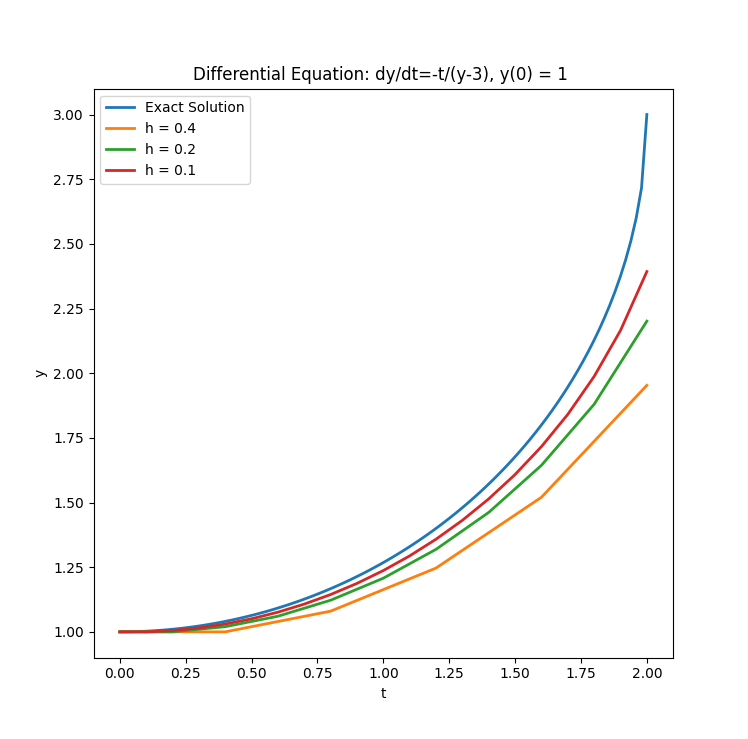
\includegraphics[width=0.8\textwidth]{plot_euler.png}
  \caption{Explicit Euler approximation with jump step \( h = 0.4 \), \( h = 0.2 \), and \( h = 0.1 \)}
\end{figure}

\subsubsection{Fourth-order Runge-Kutta}
Alternatively, we can use RK4 to approximate the values of the exact solution, the process is performed as follows:
First, we have \( (t_0, y_0) = (0, 1) \). Then, the calculation of \( y_1 \) is based on \( y_0 \) with:
\begin{alignat*}{4}
  k_1 & = f(t_0, y_0)                                            &  & = f(0, 1)                    &  & = 0                   \\
  k_2 & = f \left(t_0 + \frac{h}{2}, y_0 + k_1\frac{h}{2}\right) &  & = f(0.2, 1)                  &  & = 0.1                 \\
  k_3 & = f \left(t_0 + \frac{h}{2}, y_0 + k_2\frac{h}{2}\right) &  & = f(0.2, 1.02)               &  & = 0.10101010101010102 \\
  k_4 & = f(t_0 + h, y_0 + k_3h)                                 &  & = f(0.4, 1.0404040404040404) &  & = 0.2041237113402062
\end{alignat*}

We have
\begin{align*}
  y_1 & = y_0 + \frac{1}{6}h(k_1 + 2k_2 + 2k_3 + k_4)                                                              \\
      & = 1 + \frac{1}{6} \cdot 0.4\left(0 + 2 \cdot 0.1 + 2 \cdot 0.10101010101010102 + 0.2041237113402062\right) \\
      & \approx 1.0404095942240272
\end{align*}

The calculation of \( y_2 \) is based on \( y_1 \) with:
\begin{alignat*}{4}
  k_1 & = f(t_1, y_1)                                            &  & = f(0.4, 1.0404095942240272) &  & = 0.20412428986230166 \\
  k_2 & = f \left(t_1 + \frac{h}{2}, y_1 + k_1\frac{h}{2}\right) &  & = f(0.6, 1.0812344521964876) &  & = 0.3127010492172137  \\
  k_3 & = f \left(t_1 + \frac{h}{2}, y_1 + k_2\frac{h}{2}\right) &  & = f(0.6, 1.10294980406747)   &  & = 0.316280508173406   \\
  k_4 & = f(t_1 + h, y_1 + k_3h)                                 &  & = f(0.8, 1.1669217974933896) &  & = 0.43642437016928914
\end{alignat*}

We have
\begin{align*}
  y_2 & = y_1 + \frac{1}{6}h(k_1 + 2k_2 + 2k_3 + k_4)                                                             \\
      & = 1.0404095942240272 + \frac{1}{6} \cdot 0.4\left(0.20412428986230166 + 2 \cdot 0.3127010492172137\right. \\
      & \ \left.+\ 2 \cdot 0.316280508173406 + 0.43642437016928914\vphantom{1}\right)                             \\
      & \approx 1.1669770458782158
\end{align*}

The calculation of \( y_3 \) is based on \( y_2 \) with:
\begin{alignat*}{4}
  k_1 & = f(t_2, y_2)                                            &  & = f(0.8, 1.1669770458782158) &  & = 0.43643752425527393 \\
  k_2 & = f \left(t_2 + \frac{h}{2}, y_2 + k_1\frac{h}{2}\right) &  & = f(1, 1.2542645507292707)   &  & = 0.5728244794580668  \\
  k_3 & = f \left(t_2 + \frac{h}{2}, y_2 + k_2\frac{h}{2}\right) &  & = f(1, 1.2815419417698293)   &  & = 0.5819170245155089  \\
  k_4 & = f(t_2 + h, y_2 + k_3h)                                 &  & = f(1.2, 1.3997438556844193) &  & = 0.7498799515706484
\end{alignat*}

We have
\begin{align*}
  y_3 & = y_2 + \frac{1}{6}h(k_1 + 2k_2 + 2k_3 + k_4)                                                             \\
      & = 1.1669770458782158 + \frac{1}{6} \cdot 0.4\left(0.43643752425527393 + 2 \cdot 0.5728244794580668\right. \\
      & \ \left.+\ 2 \cdot 0.5819170245155089 + 0.7498799515706484\vphantom{1}\right)                             \\
      & \approx 1.4000304114630875
\end{align*}

The calculation of \( y_4 \) is based on \( y_3 \) with:
\begin{alignat*}{4}
  k_1 & = f(t_3, y_3)                                            &  & = f(1.2, 1.4000304114630875) &  & = 0.7500142556442817 \\
  k_2 & = f \left(t_3 + \frac{h}{2}, y_3 + k_1\frac{h}{2}\right) &  & = f(1.4, 1.5500332625919437) &  & = 0.9655393905812101 \\
  k_3 & = f \left(t_3 + \frac{h}{2}, y_3 + k_2\frac{h}{2}\right) &  & = f(1.4, 1.5931382895793296) &  & = 0.9951226830826048 \\
  k_4 & = f(t_3 + h, y_3 + k_3h)                                 &  & = f(1.6, 1.7980794846961294) &  & = 1.3312028371489164
\end{alignat*}

We have
\begin{align*}
  y_4 & = y_3 + \frac{1}{6}h(k_1 + 2k_2 + 2k_3 + k_4)                                                            \\
      & = 1.4000304114630875 + \frac{1}{6} \cdot 0.4\left(0.7500142556442817 + 2 \cdot 0.9655393905812101\right. \\
      & \ \left.+\ 2 \cdot 0.9951226830826048 + 1.3312028371489164\vphantom{1}\right)                            \\
      & \approx 1.8001998274711428
\end{align*}

The calculation of \( y_5 \) is based on \( y_4 \) with:
\begin{alignat*}{4}
  k_1 & = f(t_4, y_4)                                            &  & = f(1.6, 1.8001998274711428) &  & = 1.3335554008361483 \\
  k_2 & = f \left(t_4 + \frac{h}{2}, y_4 + k_1\frac{h}{2}\right) &  & = f(1.8, 2.0669109076383725) &  & = 1.9290762422741867 \\
  k_3 & = f \left(t_4 + \frac{h}{2}, y_4 + k_2\frac{h}{2}\right) &  & = f(1.8, 2.1860150759259804) &  & = 2.2113431671325614 \\
  k_4 & = f(t_4 + h, y_4 + k_3h)                                 &  & = f(2, 2.6847370943241673)   &  & = 6.343911586149272
\end{alignat*}

We have
\begin{align*}
  y_5 & = y_4 + \frac{1}{6}h(k_1 + 2k_2 + 2k_3 + k_4)                                                            \\
      & = 1.8001998274711428 + \frac{1}{6} \cdot 0.4\left(1.3335554008361483 + 2 \cdot 1.9290762422741867\right. \\
      & \ \left.+\ 2 \cdot 2.2113431671325614 + 6.343911586149272\vphantom{1}\right)                             \\
      & \approx 2.8640868811910707
\end{align*}

Compare \( y_i \) with the ones obtained when using the exact solution, we have the error table for RK4 method as follows:

\begin{table}[H]
  \centering
  \begin{tabular}{@{}cS[table-format=1.16]S[table-format=1.16]S[table-format=1.20]@{}}
    \toprule
    {}      & {Approximation}    & {Exact Solution}   & {Relative error (\%)}  \\
    \midrule
    \( y_0 \) & 1                  & 1                  & 0                      \\
    \( y_1 \) & 1.0404095942240272 & 1.0404082057734576 & 0.00013345248162436595 \\
    \( y_2 \) & 1.1669770458782158 & 1.166969722017664  & 0.000627596450329253   \\
    \( y_3 \) & 1.4000304114630875 & 1.4                & 0.002172247363398304   \\
    \( y_4 \) & 1.8001998274711428 & 1.8                & 0.011101526174586396   \\
    \( y_5 \) & 2.8640868811910707 & 3                  & 4.5304372936309765     \\
    \bottomrule
  \end{tabular}
\end{table}

Observe that given \( h = 0.4 \), the relative errors in the approximation are drastically smaller than Euler's. But if we want to reduce those errors further using only RK4, we must reduce the step size. Following is a graph illustrating our approximations of the exact solution using the step size of \( 0.4 \), \( 0.2 \), and \( 0.1 \). Note that, from the graph we can tell the error is reduced by a factor, that is much better than ``linear'' one, with respect to the change in \( h \), so the improvement is prominent. To be more precise, that factor is ``quartic'' with respect to the change in \( h \), or of order \( O(h^4) \).

\begin{figure}[H]
  \centering
  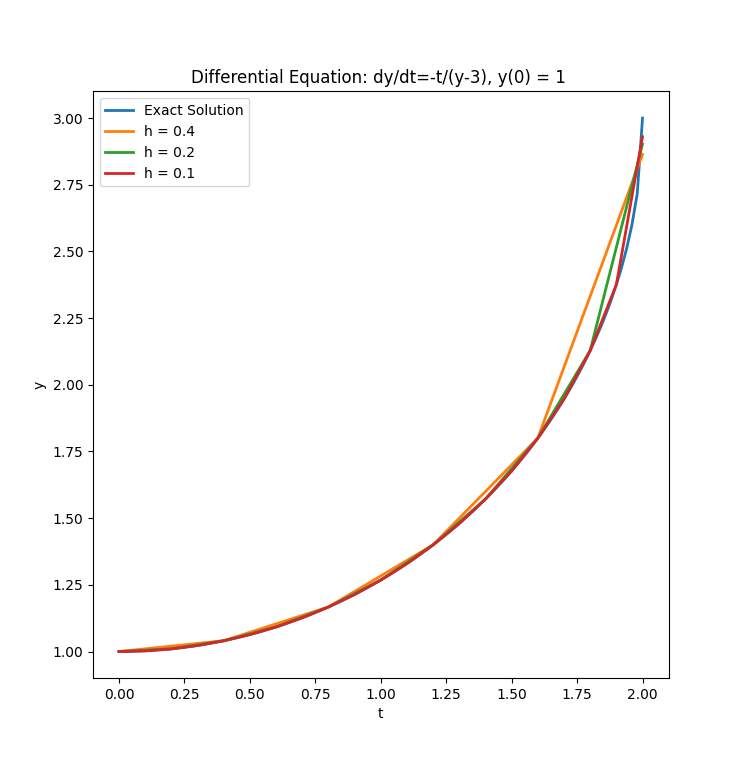
\includegraphics[width=0.9\textwidth]{plot_runge_kutta.png}
  \caption{RK4 approximation with jump step \( h = 0.4 \), \( h = 0.2 \), and \( h = 0.1 \)}
\end{figure}

Our final observation is that, despite being able to maintain a relatively less error than explicit Euler method, RK4 requires much more resources (space and time) to calculate the approximation for each time step. So there is a trade-off between predicting the values accurately and predicting them quickly.

\newpage
%%%%%%%%%%%%%%%%%%%%%%%%%%%%%%%%%
\section{Forecasting \texorpdfstring{\( CO_2 \)}{} concentration using flux}
\subsection{A \texorpdfstring{\( CO_2 \)}{} concentration model}
\subsubsection{\texorpdfstring{\( CO_2 \)}{} exchange}
To describe the concentration of \( CO_2 \) in the greenhouse air, we consider a greenhouse with thermal screens, which allow us to control light, temperature and humidity more precisely, which leads to a better climate control in the greenhouse.
\begin{figure}[H]
  \centering
  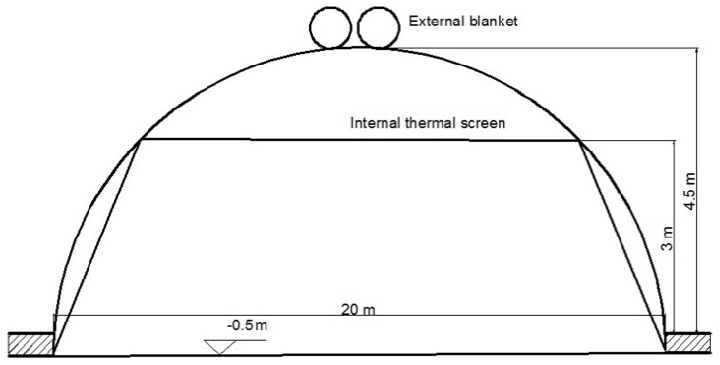
\includegraphics[width=0.9\textwidth]{thrscr.png}
  \caption{Greenhouse thermal screen}\label{fig:thrscr}
\end{figure}

In Figure~\ref{fig:thrscr}, we see that a thermal screen divides the greenhouse into two compartments, above and below the screen.
This results in different concentrations of \( CO_2 \) in the two compartments.
\begin{figure}[H]
  \centering
  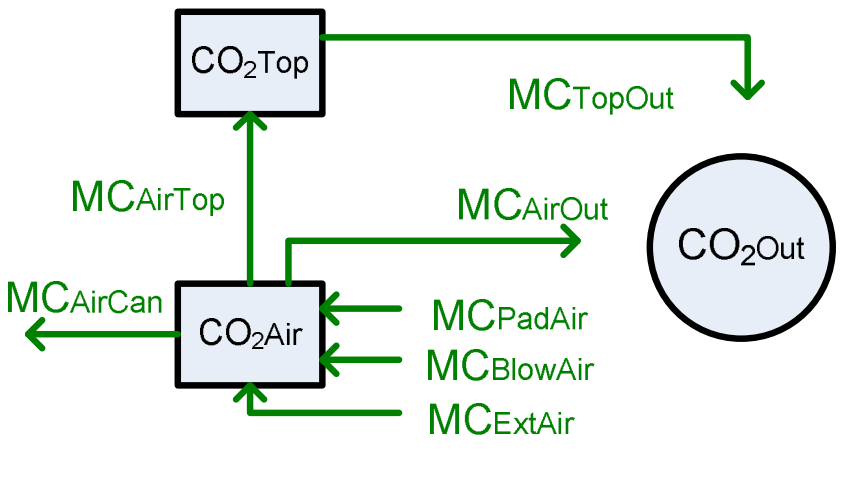
\includegraphics[width=0.8\textwidth]{CO2}
  \caption{The \( CO_2 \) flow inside and outside a greenhouse}\label{fig:CO2}
\end{figure}

All \( CO_2 \) in the model can be categorized into three \( CO_2 \) regions to calculate their respective concentrations (assume that each region has the same \( CO_2 \) concentration everywhere): \( CO_{2Top} \) which is from above the screen, \( CO_{2Air} \) which is from below the screen, and \( CO_{2Out} \) which is from outside the greenhouse.
Each relates to each other in the diagram shown in Figure~\ref{fig:CO2}.

%%%%%%%%%%
\subsubsection{Dynamical systems and assumptions}
From Figure~\ref{fig:CO2}, the fluctuation of \( CO_2 \) concentration in the lower and upper compartments of the greenhouse is represented by two differential equations:
\begin{align}
  \begin{cases}
    cap_{CO_2Air}\dot{CO_{2Air}} = MC_{BlowAir} + MC_{ExtAir} + MC_{PadAir} \\ \qquad \qquad \qquad \qquad \qquad
    - MC_{AirCan} - MC_{AirTop} - MC_{AirOut}                               \\
    cap_{CO_2Top}\dot{CO_{2Top}} = MC_{AirTop} - MC_{TopOut}
  \end{cases}
\end{align}

In which, \( cap_A, CO_{2 A}, \dot{CO_2}_A \) and \( MC_{AB} \) denote the capacity to store \( CO_2 \) in \( A \) (\( m \)), the \( CO_2 \) concentration in \( A \) (\( mg\ m^{-3} \)), the rate of change of \( CO_2 \) concentration in \( A \) (\( mg\ m^{-3}\ s^{-1} \)), and the net \( CO_2 \) flux from \( A \) to \( B \) (\( mg\ m^{-2}\ s^{-1} \)) respectively, where \( Air \) and \( Top \) represent the lower and upper compartments, \( Blow \) represents the direct air heater, \( Ext \) represents the source from the third party, \( Pad \) represents the pad system, \( Can \) represents the total foliage of the plants inside the greenhouse, and \( Out \) represents the space outside the greenhouse.

In order to solve the equations, we must consider the formulas that calculate each \( MC_{AB} \) that was presented.

The amount of \( CO_2 \) going from the direct air heater into the greenhouse air is given by taking the product of the capacity \( P_{Blow} \) (\( W \)) of the heater, the amount of \( CO_2 \) generated for each Joule of sensible heat released by the heater \( \eta_{HeatCO_2} \) (\( mg_{CO_2}\ J^{-1} \)), and the dimensionless parameter \( U_{Blow} \), then dividing it by the area of the greenhouse \( A_{Flr} \) (\( m^2 \)).
\begin{align}
  MC_{BlowAir} = \frac{\eta_{HeatCO_2}U_{Blow}P_{Blow}}{A_{Flr}}
\end{align}

Similarly, the amount of \( CO_2 \) that is pumped into the greenhouse by the third party equals the third party's ability to pump \( CO_2 \) \( \phi_{ExtCO_2} \) (\( mg\ s^{-1} \)) times the dimensionless parameter \( U_{ExtCO_2} \), then divided by the area of the greenhouse.
\begin{align}
  MC_{ExtAir} = \frac{U_{ExtCO_2}\phi_{ExtCO_2}}{A_{Flr}}
\end{align}

The amount of \( CO_2 \) that enters the greenhouse through the pad system is calculated differently.
It depends on the difference between the concentration of \( CO_2 \) inside and outside the greenhouse, and the ability of the pad system for the air to go through.
As the pad can be adjusted to let more air in, the flux of the pad \( f_{Pad} \) (\( m^{-1} \)) can be given as the product of the permeability of the pad \( U_{Pad} \) and the ability for the airflow to pass through \( \phi_{Pad} \) (\( m^3\ s^{-1} \)) divided by the area of the greenhouse floor.
\begin{equation}
  \begin{split}
    MC_{PadAir} & = f_{Pad} (CO_{2 Out} - CO_{2 Air}) \\
    & = \frac{U_{Pad} \phi_{Pad}}{A_{Flr}} (CO_{2 Out} - CO_{2 Air})
  \end{split}
\end{equation}

The calculation of the net flux of \( CO_2 \) from the lower compartment to the upper compartment of the greenhouse is more complicated.
It depends on the difference in temperature and air density between the two compartments and the airflow rate through the thermal screen \( f_{ThScr} \) (\( m\ s^{-1} \)).
\begin{align}
  MC_{AirTop} = f_{ThScr} (CO_{2 Air} - CO_{2 Top})
\end{align}

Furthermore, \( f_{ThScr} \) is given by
\begin{multline}
  f_{ThScr} = U_{ThScr} K_{ThScr} |T_{Air} - T_{Top}|^{\frac{2}{3}} \\
  + (1 - U_{ThScr}) {\left[\frac{g(1 - U_{ThScr})}{2\rho^{Mean}_{Air}} |\rho_{Air} - \rho_{Top}|\right]}^{\frac{1}{2}}
\end{multline}

To calculate the the airflow rate, we consider the screen and the open regions separately, with \( U_{ThScr} \in [0,1] \) representing the percentage of places that are covered by the thermal screen. The flux through the screen depends on the difference between the temperature above and below the screen and the permeability of the screen \( K_{ThScr} \) (\( m\ K^{-\frac{2}{3}}\ s^{-1} \)).

At places that are not covered by the thermal screen, the flux is given by the Navier-Stokes equation depending on the difference of the air density below the screen \( \rho_{Air} \) and the air density above the screen \( \rho_{Top} \) (\( kg\ m^{-3} \)).

The net \( CO_2 \) flux from the inside to the outside of the greenhouse is given by the following formula
\begin{align}
  MC_{AirOut} = (f_{VentSide} + f_{VentForced})(CO_{2 Air} - CO_{2 Out})
\end{align}

The flux \( f_{VentSide} \) and \( f_{VentForced} \) (\( m s^{-1} \)) are respectively the flux due to the fan system on the sidewalls and the fan system inside the greenhouse.
%In this case, we should consider the Bernoulli principle in representing the pressure difference outside and inside of the greenhouse.
\begin{multline}
  \label{eq:vent_roof_side}
  f_{VentRoofSide} = \frac{C_d}{A_{Flr}} \left[\frac{U_{Roof}^2 U_{Side}^2 A_{Roof}^2 A_{Side}^2}{U_{Roof}^2 A_{Roof}^2 + U_{Side}^2 A_{Side}^2} \cdot \frac{2gh_{SideRoof} (T_{Air} - T_{Out})}{T_{Air}^{Mean}}\right. \\
  + \left.{ \left(\frac{U_{Roof} A_{Roof} + U_{Side} A_{Side}}{2}\right)}^2 + C_W v_{Wind}^2\right]^{\frac{1}{2}}
\end{multline}

The above formula is the sum of the two components multiplied with the ratio between the discharged coefficient \( C_d \) and the area of the greenhouse \( A_{Flr} \) (\( m^2 \)).

The first component represents the Stack effect when the ventilation area on the roof \( A_{Roof} \) (\( m^2 \)) is non-zero. Stack effect happens when there exists a temperature difference between the interior and exterior of the building. In this case, the first component in the formula is given based on the equation of the Stack effect, that is caused by the temperature difference between the outside and inside of the greenhouse (the space under the thermal screen).
The second component is given by the pressure difference inside and outside the greenhouse. The pressure from the outside of the greenhouse is caused by the natural airflow through the roof surface, while the pressure from the inside of the greenhouse is caused by the lateral airflow. Furthermore, the pressure difference can be calculated as the total area of the ventilation openings on the greenhouse divided by two times the natural wind speed \( v_{Wind} \) (\( m\ s^{-1} \)) squared and the global wind pressure coefficient \( C_w \) (dimensionless) based on the Bernoulli principle.

In the presence of an insect screen, the movement speed of the air currents through the ventilation areas will be reduced by a factor of \( \eta_{InsScr} \), where \( \zeta_{InsScr} \) is the porosity, the ratio of the area of the holes in the screen to the total area of the screen.
\begin{align}
  \eta_{InsScr} = \zeta_{InsScr} (2 -  \zeta_{InsScr})
\end{align}

Given the leakage coefficient \( c_{leakage} \), which depends on the greenhouse type and is dimensionless, an amount of approximately half the leakage rate is added to the air-exchange rate, where leakage rate is calculated as below.
\begin{align}
  f_{leakage} = \begin{cases}
    0.25 \cdot c_{leakage}     & \text{if~} v_{Wind} < 0.25    \\
    v_{Wind} \cdot c_{leakage} & \text{if~} v_{Wind} \geq 0.25
  \end{cases}
\end{align}

Let \( \eta_{Side\_Thr} \) be the Stack-effect threshold. If \( \eta_{Side} \), the ratio between the sidewalls ventilation
area and the total ventilation area, exceeds the threshold, the Stack effect does not occur and vice versa. Then, \( f_{VentSide} \) is given by the following
\begin{gather}
  f_{VentSide} =
  \begin{cases}
    \eta_{InsScr} f''_{VentSide} + 0.5f_{leakage} & \text{if~} \eta_{Side} \geq \eta_{Side\_Thr} \\
    \begin{split}
      & \eta_{InsScr} [U_{ThScr}f''_{VentSide} + (1-U_{ThScr}) \\
      & \qquad f_{VentRoofSide} \eta_{Side}] + 0.5 f_{leakage}
    \end{split}                    & \text{if~} \eta_{Side} < \eta_{Side\_Thr}
  \end{cases}
\end{gather}

In which,  \( f''_{VentSide} \) is  \( f_{VentSide} \) when \( A_{Roof} = 0 \).
Moreover, the Stack effect does not occur where is covered by the thermal screen.

The flux \( f_{VentForced} \) by the fan system inside the greenhouse is calculated as follows.
\begin{align}
  f_{VentForced} = \frac{\eta_{InsScr} U_{VentForced} \phi_{VentForced} } {A_{Flr}}
\end{align}

The dimensionless parameter \( U_{VentForced} \in [0,1] \) is to adjust the wind speed \( \phi_{VentForced} \) due to
the system (\( m^3\ s^{-1} \)).

Similarly to \( MC_{AirOut} \), the net \( CO_2 \) flux from the greenhouse to outside the greenhouse through the roof openings is calculated by using the formula below, where \( f_{VentRoof} \) is the flux rate through the roof openings.
\begin{align}
  MC_{TopOut} = f_{VentRoof}(CO_{2 Top} - CO_{2 Out})
\end{align}

\( f_{VentRoof} \) is the flux rate openings and is given by
\begin{gather}
  f_{VentRoof} =
  \begin{cases}
    \eta_{InsScr} f''_{VentRoof} + 0.5f_{leakage} & \text{if~} \eta_{Roof} \geq \eta_{Roof\_Thr} \\
    \begin{split}
      & \eta_{InsScr} [U_{ThScr}f''_{VentRoof} + (1-U_{ThScr}) \\
      & \qquad f_{VentRoofSide} \eta_{Side}] + 0.5 f_{leakage}
    \end{split}                    & \text{if~}  \eta_{Roof} < \eta_{Roof\_Thr}
  \end{cases}
\end{gather}

% check again part
However, when the ratio of the roof-opening area to the total ventilation area exceeds the Stack-effect threshold, the Stack effect does not occur and we cannot reuse the formula~\eqref{eq:vent_roof_side} where \( A_{Side} = 0 \) to
calculate \( f''_{VentRoof} \).
\begin{align}
  f''_{VentRoof} = \frac{C_d U_{Roof} A_{Roof}}{2A_{Flr}} {\left[\frac{gh_{Roof}(T_{Air} - T_{Out})}{2T^{Mean}_{Air}} + C_w v^2_{Wind}\right]}^{ \frac{1}{2}}
\end{align}

Finally, we need to consider the amount of \( CO_2 \) absorbed into the leaves due to photosynthesis.
\begin{align}
  MC_{AirCan} = M_{CH_2O} h_{C_{Buf}} (P - R)
\end{align}

Here, \( M_{CH_2O} \) is the molar mass of \( CH_2O \) (\( mg\ \mu mol^{-1} \)), \( P \) is the photosynthetic rate (\( \mu mol_{CO_2}\ m^{-2}\ s{-1} \)), \( R \) is the respiration rate (\( \mu mol_{CO_2}\ m^{-2}\ s^{-1} \)), and \( h_{C_{Buf}} \) shows the cessation of photosynthesis when \( CH_2O \) is \( C_{Buf} \) (\( mg\ m^{-2} \)) has reached \( C_{Max} \) (\( mg\ m^{-2} \)), which is the limit of the carbohydrates storage of the plants. The respiration rate during this process is usually as about \( 1\% \) of the photosynthesis rate, and thus can be omitted during further calculation. The photosynthesis rate is described in more detail in Section~\ref{sssec:photo_c3}.

%%%%%%%%%%%
\subsubsection{A model of photosynthesis of C3 plants}\label{sssec:photo_c3}
Photosynthesis, the process by which green plants and certain other organisms transform light energy into chemical energy. During photosynthesis in green plants, light energy is captured and used to convert water, carbon dioxide, and minerals into oxygen and energy-rich organic compounds.

Photosynthesis has two phases: light-dependent phase and light-independent (or dark) phase.

The photosynthetic rate \( P \) is defined as the diffusion of \( CO_2 \) from air into the leaf cells through stomata. From Fick's law for gas diffusion, we construct:
\begin{align}
  \label{eq:photo_co2}
  P = \frac{CO_{2Air} - CO_{2Stom}}{Res}
\end{align}

The notation \( CO_{2Stom} \) is the concentration of \( CO_2 \) in the stomata (\( \mu mol\ m^{-3} \)) and \( Res \) is the resistance-to-absorption coefficient (\( s\ m^{-1} \)).

This way of calculating photosynthetic rate \( P \) is different from the model of Vanthoor 2011. In there the author uses:
\begin{align}
  P = \frac{J \cdot (CO_{2Stom} - \Gamma)}{4 \cdot (CO_{2Stom} + 2\Gamma)}
\end{align}
where \( J \) (\( \mu mol \{e^-\} m^{-2} s^{-1} \)) is the electron transport rate, 4 (\( \mu mol \{e^-\} \mu mol^{-1} \{CO_2\} \)) is the
number of electrons per fixed \( CO_2 \) molecule, \( CO_{2Stom} \) (\( \mu mol\{CO_2\}\ mol^{-1}\{air\} \)) is the \( CO_2 \) concentration in the stomata and \( \Gamma \) (\( \mu mol \{CO_2\} mol^{-1} \{air\} \)) is the \( CO_2 \) compensation point.

Following by the photorespiration \( R \):
\begin{align}
  R = P \cdot \frac{\Gamma}{CO_{2Stom}}
\end{align}

But since we do not consider electron transport rate, we will use equation~\eqref{eq:photo_co2} constructed from Fick's law combined with Michaelis-Menten model.

In the dark phase, through Michaelis-Menten relationship describing enzyme-substrate reaction, the photosynthetic rate is given by:
\begin{align}
  \label{eq:photo_dark}
  P = \frac{P_{Max} \cdot CO_{2Stom}}{CO_{2\ 0.5} + CO_{2Stom}}
\end{align}
where \( CO_{2\ 0.5} \) is the concentration of \( CO_2 \) in the substrate when \( P = P_{Max}/2 \) (\( \mu mol\ m^{-3} \)).

From~\eqref{eq:photo_co2} and~\eqref{eq:photo_dark}, we form a quadratic equation for the rate of photosynthetic \( P \). The photosynthetic rate \( P \) then no longer depends on the concentration of \( CO_2 \) in the stomata but only on the concentration of \( CO_2 \) in the air, the resistance coefficient \( Res \), and the maximum photosynthetic rate.
\begin{align}
  \label{eq:resist_photo}
  ResP^2 - (CO_{2Air} + CO_{2\ 0.5} + ResP_{Max})P + CO_{2Air}P_{Max} = 0
\end{align}

Solving equation~\eqref{eq:resist_photo} requires \( P_{Max} \) to be obtained. For the model for the photosynthesis of one leaf unit, the maximum photosynthetic rate is usually be found through the Arrhenius model.
\begin{align}
  \label{eq:photo_rate}
  k(T) = k(T_0)\exp \left(-\frac{H_a}{R} \left(\frac{1}{T} - \frac{1}{T_0}\right)\right)
\end{align}
where \( k(T) \) is the reaction rate at \( T(K) \), \( T_0 \) is the optimum temperature for which the reaction
rate is known (\( K \)), \( H_a \) is the activation energy for the reaction (\( J\ mol^{-1} \)), and \( R \) is the ideal gas constant.

Yet a problem is raised when the temperature increases to a certain threshold, the enzyme activity will be inhibited and the photosynthesis is slowed down and cease to advance. A model represents the activity of the Rubisco enzyme during photosynthesis with temperature as its parameter.
\begin{align}
  \label{eq:rubisco}
  f(T) = \frac{1 + \exp \left(-\frac{H_d}{R} \left(\frac{1}{T_0} - \frac{1}{\frac{H_d}{S}}\right)\right)}{1 + \exp \left(-\frac{H_d}{R}\left(\frac{1}{T} - \frac{1}{\frac{H_d}{S}}\right)\right)}
\end{align}
In the model~\eqref{eq:rubisco}, \( f(T) \) represents the enzyme activity at \( T(K) \), \( H_d \) is the deactivation energy (\( J\ mol^{-1} \)), and \( S \) is the corresponding entropy quantity (\( J\ mol^{-1}\ K^{-1} \)).

Combining~\eqref{eq:photo_rate} and~\eqref{eq:rubisco}, we obtain the formula for maximum rate of photosynthetic rate.
\begin{align}
  \label{eq:photo_max}
  P_{Max}(T) = k(T)f(T)
\end{align}

For a photosynthesis for the whole canopy, considering \( LAI \) (leaf area index), due to Beer's law, the intensity of the transmitted beam \( I \) with the initial state is \( I_0 \) (\( \mu mol\{photons\}\ m^{-2}\ s^{-1} \)) is equal to
\begin{align}
  I = \frac{I_0 \cdot K \cdot \exp \left(-K \cdot LAI\right)}{1 - m}
\end{align}

If the leaves are horizontally stratified such as in the case of tomato, the dimensionless extinction coefficient \( K \) will be between 0.7 and 1.0. Meanwhile, if the leaves are sloped as in the case of wet rice, \( K \) will be between 0.3 and 0.5. \( m \) is the transmittance coefficient of the leaves which is set as \( 0.1 \).

The amount of light absorbed by the canopy can be measured as the difference in the intensity of the light ray before entering the foliage and after passing through the foliage
\begin{align}
  L =L_0 \left(1 - \frac{K \cdot \exp \left(-K \cdot LAI\right)}{1 - m}\right)
\end{align}

In this formula, \( L \) is luminous flux received by the leaves per unit area of the greenhouse floor (\( \mu mol\{photons\}\ m^{-2}\ s^{-1} \)) and \( L_0 \) is the initial value of \( L \).

For calculating the maximum photosynthetic rate of all leaves in the greenhouse, we apply the modified Arrhenius model.
\begin{align}
  \label{eq:photo_rate_mod}
  k(T) = LAI \cdot k(T_0) \cdot \exp \left(-\frac{H_a}{R} \left(\frac{1}{T} - \frac{1}{T_0}\right)\right)
\end{align}

Here, \( k(T) \) is the reaction rate for the whole canopy at \( T(K) \) and \( k(T_0) \) is the reaction rate under the optimal condition \( T_0 \) \( K \) of one leaf unit.

Unlike the photosynthesis model for one leaf unit, the amount of light energy absorbed into the foliage in response to \( LAI \) needs to be added since it affects the maximum photosynthetic rate \( P_{Max} \). Therefore, we consider the following formula of \( P_{Max} \), which is a dependent function on \( L \) and \( T \).
\begin{align}
  P_{Max} (L,T) = \frac{P_{MLT} \cdot P_{Max}(T) \cdot L}{L + L_{0.5}}
\end{align}

In which, \( L_{0.5} \) is light intensity when \( P_{Max} (L,T) = P_{Max}(T)/2 \) (\( \mu mol\{photons\}\ m^{-2}\ s^{-1} \))
\( P_{Max}(T) \) is calculated by using the formula~\eqref{eq:photo_max} with \( k(T) \) as in~\eqref{eq:photo_rate_mod}, and \( P_{MLT} \) are the maximum
photosynthetic rate at the point of light saturation and the optimal temperature \( T \).

\subsubsection{Vanthoor 2011 model of photosynthesis}
For calculating photosynthesis rate and respiration rate, we implement through the photosynthesis model described in Vanthoor 2011.

The photosynthesis rate is calculated through:
\begin{align}
  P = \frac{J \cdot (CO_{2Stom} - \Gamma)}{4 \cdot (CO_{2Stom} + 2\Gamma)}
\end{align}
where \( J \) (\( \mu mol\{e^-\}\ m^{-2}\ s^{-1} \)) is the electron transport rate, \( 4 \) (\( \mu mol \{e^-\}\ \mu mol^{-1} \{CO_2\} \)) is the number of electrons per fixed \( CO_2 \) molecule, \( CO_{2Stom} \) (\( \mu mol\{CO_2\}\ mol^{-1}\{air\} \)) is the \( CO_2 \) concentration in the stomata and \( \Gamma \) (\( \mu mol \{CO_2\}\ mol^{-1} \{air\} \)) is the \( CO_2 \) compensation point.

Following by the photorespiration \( R \):
\begin{align}
  R = P \cdot \frac{\Gamma}{CO_{2Stom}}
\end{align}

The electron transport rate, J, is a function of the potential rate of electron transport and of the absorbed \( PAR \) by the canopy:

\begin{align}
  J = \frac{J^{POT} + \alpha PAR_{can} - {\sqrt{{(J^{POT} + \alpha PAR_{can})}^2 - 4\Theta\cdot J^{POT}\cdot \alpha PAR_{can}}}}{2 \Theta}
\end{align}
where \( J^{POT} \) (\( \mu mol\{e^-\}\ m^{-2}\ s^{-1} \)) is the potential rate of electron transport, \( PAR_{Can} \) (\( PAR \) by the canopy) (\( \mu mol\{photons\}\ m^{-2}\ s^{-1} \)) is the absorbed \( PAR \), \( \alpha \) (\( \mu mol\{e^-\}\ \mu mol^{-1}\{photons\} \)) is the conversion factor from photons to electrons, including an efficiency term, and \( \Theta \) (\( - \)) is the degree of curvature of the electron transport rate.

The potential rate of electron transport \( J^{POT} \), depends on temperature:

\begin{align}
  J^{POT} = J^{MAX}_{25,Can} \cdot \exp \left(E_j\frac{T_{Can,K}-T_{25,K}}{R\cdot T_{Can,K}\cdot T_{25,K}}\right) \cdot \frac{1 + \exp \left(\frac{S\cdot T_{25,K}-H}{R\cdot T_{25,K}}\right)}{1 + \exp \left(\frac{S\cdot T_{Can,K}-H}{R\cdot T_{Can,K}}\right)}
\end{align}
where \( J^{MAX}_{25,Can} \) (\( \mu mol \{e^-\}\ m^{-2}\ s^{-1} \)) is the maximum rate of electron transport at \( 25 \celsius \) for the canopy, \( E_j \) (\( J\ mol^{-1} \)) is the activation energy for \( J^{POT} \), \( T_{Can,K} \) (\( K \)) is the canopy temperature, \( T_{25,K} \) (\( K \)) is the reference temperature at \( 25 \celsius \), \( R \) (\( J\ mol^{-1}\ K^{-1} \)) is the molar gas constant, \( S \) (\( J\ mol^{-1}\ K^{-1} \)) is the entropy term and \( H \) (\( J\ mol^{-1} \)) is the deactivation energy.

The maximum rate of electron transport at \( 25 \celsius \) for the canopy is calculated by:
\begin{align}
  J^{MAX}_{25,Can} = LAI \cdot J^{MAX}_{25,Leaf}
\end{align}
where \( J^{MAX}_{25,Leaf} \), (\( \mu mol\{e^-\}\ m^{-2}\{leaf\}\ s^{-1} \)) is the maximum rate of electron transport for the leaf at \( 25 \celsius \).

The total \( PAR \) absorbed by the canopy is the sum of the \( PAR \) transmitted by the greenhouse cover that is directly absorbed, and the \( PAR \) reflected by the greenhouse floor that is indirectly absorbed:
\begin{align}
  PAR_{Can} = PAR_{GhCan} + PAR_{FlrCan}
\end{align}

The \( PAR \) which is directly absorbed by the canopy is described by a negative exponential decay of light with \( LAI \) in a homogeneous crop:
\begin{align}
  PAR_{GhCan} = PAR_{Gh}\cdot (1-\rho_{can})\cdot(1 - \exp \left(-K_1\cdot LAI\right))
\end{align}
where \( PAR_{Gh} \) (\( \mu mol \{photons\}\ m^{-2}\ s^{-1} \)) is the \( PAR \) above the canopy, \( \rho_{can} \) (\( - \)) is the reflection coefficient of the canopy for \( PAR \) and \( K_1 \) is the extinction coefficient of the canopy for \( PAR \) (\( - \)).

The PAR above the canopy is described by:
\begin{align}
  PAR_{Gh} = \tau_{Gh} \cdot \eta_{Glob\_PAR}\cdot I_{Glob}
\end{align}
where \( \tau_{Gh} \) (\( - \)) is the light transmission of the greenhouse cover \( \eta_{Glob\_PAR} \) \\    (\( \mu mol\{photons\}\ J^{-1} \)) is a conversion factor from global radiation to \( PAR \) and \( I_{Glob} \) (\( W\ m^{-2} \)) is the outside global radiation.

Absorption of \( PAR \) reflected by the greenhouse floor is described by:
\begin{align}
  PAR_{FlrCan} = \rho_{Flr}PAR_{Gh}\cdot (1-\rho_{Can})\cdot \exp \left(K_1\cdot LAI\right) \cdot (1 - \exp \left(K_2\cdot LAI\right))
\end{align}
where \( \rho_{Flr} \) (\( - \)) is the reflection coefficient of the greenhouse floor and \( K_2 \) (\( - \)) is the extinction coefficient of the canopy when \( PAR \) is reflected from the floor to the canopy. We assumed \( K_2 \) to be equal to \( K_1 \).

The \( CO_2 \) concentration inside the stomata, \( CO_{2Stom} \) depends on the stomatal and mesophyll conductance, boundary layer resistance, the photosynthesis rate and the difference between the \( CO_2 \) concentration in the stomata and the \( CO_2 \) concentration of the greenhouse air. However, the \( CO_2 \) concentration in the stomata is assumed to be a fixed fraction of the \( CO_2 \) concentration in the greenhouse air:
\begin{align}
  CO_{2Stom} = \eta_{CO_{2Air\_Stom}} \cdot CO_{2Air}
\end{align}
where \( \eta_{CO_{2Air\_Stom}} \) is conversion factor from the \( CO_2 \) concentration of the greenhouse air, \( CO_{2Air} \), to the \( CO_2 \) concentration in the stomata.

The \( CO_2 \) compensation point (\( \Gamma \)) affects the leaf photosynthesis rate and depends on temperature. To avoid unrealistically low optimal canopy temperatures, the sensitivity of the compensation point to temperature was adjusted by making the slope dependent of the ratio of \( J^{MAX}_{25,Leaf} \) and \( J^{MAX}_{25,Can} \):
\begin{align}
  \Gamma = \frac{J^{MAX}_{25,Leaf}}{J^{MAX}_{25,Can}}c_{\Gamma} T_{Can} + 20 c_{\Gamma} \left(1-\frac{J^{MAX}_{25,Leaf}}{J^{MAX}_{25,Can}}\right)
\end{align}
where \( c_{\Gamma} \) (\( \mu mol\{CO2\}\ mol^{-1}\{air\}\ K^{-1} \)) determines the effect of canopy temperature on the \( CO_2 \) compensation point. The right term of the equation above is introduced to assure that, for all values of \( J^{MAX}_{25,Can} \) at a temperature of \( 20 \celsius \).

\newpage
\subsection{Implementing the programs}
To calculate \( \dot{CO_{2 Air}} \) and \( \dot{CO_{2 Top}} \), we use the following \( dx \) function. Each of the \( MC \) formula will be given and explained further below. The variables are defined and used more precisely in the program attached with the report, the following is only a summary of the program.

\begin{mdframed}[leftline=false,rightline=false,backgroundcolor=magenta!10,nobreak=true]
  \begin{minted}[linenos,breaklines,breaksymbolleft=,obeytabs=true,tabsize=2]{Python}
def dx_CO2(self, t, CO2_Air, CO2_Top):
    # Equation (1) and (2) in pdf
    # Update environment variable at time t (s)
    self.update(data_Tair[int(t / 300)], data_Tout[int(t / 300)], wind_speed[int(t / 300)])

    self.CO2_Air = CO2_Air
    self.CO2_Top = CO2_Top

    return (self.MC_BlowAir() + self.MC_ExtAir() + self.MC_PadAir() - self.MC_AirCan() - self.MC_AirTop() - self.MC_AirOut()) / self.cap_CO2Air, 
    (self.MC_AirTop() - self.MC_TopOut()) / self.cap_CO2Top
  \end{minted}
\end{mdframed}

\( MC_{BlowAir} \) is assumed to be zero in this assignment.
Since \( P_{Blow} \) is assumed to be zero, this results in \( H_{BlowAir} = 0 \).
\begin{mdframed}[leftline=false,rightline=false,backgroundcolor=magenta!10,nobreak=true]
  \begin{minted}[linenos,breaklines,breaksymbolleft=,obeytabs=true,tabsize=2]{Python}
def MC_BlowAir(self):  # this Assignment assumes MC_BLowAir is zero
    # (P_Blow = 0)
    # Equation (3) in pdf
    H_BlowAir = self.H_BlowAir()
    return ETA_HEATCO2 * H_BlowAir
    
def H_BlowAir(self):
    # Equation  8.53
    return U_Blow * P_Plow / A_Flr
  \end{minted}
\end{mdframed}

\( MC_{ExtAir} \) is calculated as the equation given above.
\begin{mdframed}[leftline=false,rightline=false,backgroundcolor=magenta!10,nobreak=true]
  \begin{minted}[linenos,breaklines,breaksymbolleft=,obeytabs=true,tabsize=2]{Python}
def MC_ExtAir(self):
    # Equation (4) in pdf
    return self.U_ExtAir * self.phi_ExtCO2 / self.floor_area
  \end{minted}
\end{mdframed}

\( MC_{PadAir} \) is given as the product of \( f_{Pad} \) and the difference in the concentration of \( CO_2 \) inside and outside the greenhouse. However, in our model, we do not consider the pad so \( f_{Pad} \) is assumed to be zero.
\begin{mdframed}[leftline=false,rightline=false,backgroundcolor=magenta!10,nobreak=true]
  \begin{minted}[linenos,breaklines,breaksymbolleft=,obeytabs=true,tabsize=2]{Python}
def MC_PadAir(self):
    # Equation (5) in pdf
    # do not have PadAir with our model
    f_Pad = self.f_Pad()
    return f_Pad * (self.CO2_Out - self.CO2_Air)
    
def f_Pad(self):
    return U_Pad * phi_Pad / A_Flr
  \end{minted}
\end{mdframed}

\( MC_{AirTop} \) is calculated using air flux, with \( f \) being \( f_{ThScr} \).
\begin{mdframed}[leftline=false,rightline=false,backgroundcolor=magenta!10,nobreak=true]
  \begin{minted}[linenos,breaklines,breaksymbolleft=,obeytabs=true,tabsize=2]{Python}
def MC_AirTop(self):
    # Equation (6) in pdf
    f_ThScr = self.f_ThScr()
    return self.air_flux(f_ThScr, self.CO2_Air, self.CO2_Top)
    
def air_flux(self, f, CO2_from, CO2_to):
    # Equation 8.46
    return f * (CO2_from - CO2_to)
    
def f_ThScr(self):
    # Equation (7) in pdf
    p_Air = self.air_density()
    pressure = 101325 * (1 - 2.5577e-5 * self.elevation_height) ** 5.25588
    p_Out = M_AIR * pressure / ((self.T_Top + 273.15) * M_GAS)
    p_Mean = (p_Air + p_Out) / 2

    return U_ThScr * K_ThScr * abs(T_Air - T_Out) ** 0.66 + (1 - U_ThScr) / p_Mean * math.sqrt(0.5 * p_Mean * (1 - U_ThScr) * GRAVITY * abs(p_Air - p_Out))
  \end{minted}
\end{mdframed}

To calculate \( MC_{AirOut} \), we must calculate \( f_{VentSide} \) and \( f_{VentForced} \) separately.
In this assignment, \( f_{VentForced} \) is assumed to be 0, while \( f_{VentSide} \) is given by the following functions.

\begin{mdframed}[leftline=false,rightline=false,backgroundcolor=magenta!10,nobreak=true]
  \begin{minted}[linenos,breaklines,breaksymbolleft=,obeytabs=true,tabsize=2]{Python}
def MC_AirOut(self):
    # Equation (9) in pdf
    f_VentSide = self.f_VentSide()
    f_VentForced = self.f_VentForced()
    f_AirOut = f_VentSide + f_VentForced
    return self.air_flux(f_AirOut, self.CO2_Air, self.CO2_Out)
    
def f_VentSide(self):
    # Equation (13) in pdf
    eta_Side = 0
    eta_Roof = 1
    eta_InsScr = self.eta_InsScr_()
    d2_f_VentSide = self.d2_f_VentSide()
    d2_f_VentRoofSide = self.d2_f_VentRoofSide()
    f_leakage = self.f_leakage()
    U_ThScr = self.U_ThScr

    if eta_Side >= ETA_ROOF_THR:
        return eta_InsScr * d2_f_VentSide + 0.5 * f_leakage
    else:
        return eta_InsScr * (U_ThScr * d2_f_VentSide + 
        (1 - U_ThScr) * d2_f_VentRoofSide * eta_Side) + 0.5 * f_leakage
  \end{minted}
\end{mdframed}

Particularly, \( f''_{VentSide} \) and \( f_{VentRoofSide} \) is given below.
\begin{mdframed}[leftline=false,rightline=false,backgroundcolor=magenta!10,nobreak=true]
  \begin{minted}[linenos,breaklines,breaksymbolleft=,obeytabs=true,tabsize=2]{Python}
def d2_f_VentSide(self):
    # Equation (10) in pdf with A_roof = 0
    return 0.5 * C_d * AU_Side * v_Wind / A_Flr * math.sqrt(C_w)
    
def d2_f_VentRoofSide(self):
    # Equation (10) in pdf
    return C_d / A_Flr * math.sqrt((AU_Roof * AU_Side / math.sqrt(AU_Roof ** 2 + AU_Side ** 2)) ** 2 * (
            2 * GRAVITY * h_SideRoof * (T_Air - T_Out) / (T_Mean + 273.15)) + 0.25 * (AU_Roof + AU_Side) ** 2 * C_w * v_Wind ** 2)
  \end{minted}
\end{mdframed}

\( MC_{TopOut} \) is calculated similarly using air\_flux function with \( f_{VentRoof} \).
\begin{mdframed}[leftline=false,rightline=false,backgroundcolor=magenta!10,nobreak=true]
  \begin{minted}[linenos,breaklines,breaksymbolleft=,obeytabs=true,tabsize=2]{Python}
def MC_TopOut(self):
    # Equation (15) in pdf
    f_VentRoof = self.f_VentRoof()
    return self.air_flux(f_VentRoof, self.CO2_Top, self.CO2_Out)
  \end{minted}
\end{mdframed}

\begin{mdframed}[leftline=false,rightline=false,backgroundcolor=magenta!10,nobreak=true]
  \begin{minted}[linenos,breaklines,breaksymbolleft=,obeytabs=true,tabsize=2]{Python}
def f_VentRoof(self):
    # Equation (16) in pdf
    eta_Roof = 1  # Note: line 606 / setGlAux / GreenLight
    
    if eta_Roof >= ETA_ROOF_THR:
        return eta_InsScr * d2_f_VentRoof + 0.5 * f_leakage
    else:
        return eta_InsScr * (U_ThScr * d2_f_VentRoof + (1 - U_ThScr) * d2_f_VentRoofSide * eta_Roof) + 0.5 * f_leakage
  \end{minted}
\end{mdframed}

Finally, we calculate \( MC_{AirCan} \).
\begin{mdframed}[leftline=false,rightline=false,backgroundcolor=magenta!10,nobreak=true]
  \begin{minted}[linenos,breaklines,breaksymbolleft=,obeytabs=true,tabsize=2]{Python}
def MC_AirCan(self):
    # Equation (18) in pdf
    h_AirCan = 1  # Consider Photosynthesis always happen
    P = self.photosynthesis_rate()
    R = self.photorespiration()
    return M_CH2O * h_AirCan * (P - R)
  \end{minted}
\end{mdframed}

Electron transport rate, \( CO_{2 Stom} \), gamma are calculated using functions supporting the model in [Van11].
\begin{mdframed}[leftline=false,rightline=false,backgroundcolor=magenta!10,nobreak=true]
  \begin{minted}[linenos,breaklines,breaksymbolleft=,obeytabs=true,tabsize=2]{Python}
def photosynthesis_rate(self):
    # Equation 9.12
    J = self.electron_transport_rate()
    CO2_Stom = self.CO2_Stom()
    gamma = self.gamma()
    return 0.25 * J * (CO2_Stom - gamma) / (CO2_Stom + 2 * gamma)
    
def photorespiration(self):
    P = self.photosynthesis_rate()
    gamma = self.gamma()
    CO2_Stom = self.CO2_Stom()
    return P * gamma / CO2_Stom
  \end{minted}
\end{mdframed}

\newpage
%%%%%%%%%%%%%%%%%%%%%%%%%%%%%%%%%
\section{Testing the programs}
The data used in this model is based on climate of Texas in United States and the photosynthesis is based on tomatoes. We will consider the first step (\( t = 0 \)) where the values of the initial state are: \( CO_{2Air} = CO_{2Top} = 440 \).
\begin{itemize}
  \item \textbf{Function \texttt{MC\_BlowAir()} is equivalent to equation:}
        \begin{align*}
          MC_{BlowAir} = \frac{\eta_{HeatCO_2}U_{Blow}P_{Blow}}{A_{Flr}}
        \end{align*}

        \begin{table}[H]
          \centering
          \begin{tabular}{@{}lS@{}}
            \toprule
            \textbf{Variable}   & \textbf{Value} \\
            \midrule
            \( \eta_{HeatCO_2} \) & 0.057          \\
            \( U_{Blow} \)        & 1              \\
            \( P_{Blow} \)        & 0              \\
            \( A_{Flr} \)         & 70000          \\
            \bottomrule
          \end{tabular}
        \end{table}

  \item[-] Because we do not consider fan system inside the greenhouse, \( P_{Blow} = 0 \).
  \item[-] Result of this equation: \( MC_{BlowAir} = 0.0 \)

  \item \textbf{Function \texttt{MC\_ExtAir()} is equivalent to equation:}
        \begin{align*}
          MC_{ExtAir} = \frac{U_{ExtCO_2}\phi_{ExtCO_2}}{A_{Flr}}
        \end{align*}

        \begin{table}[H]
          \centering
          \begin{tabular}{@{}lS@{}}
            \toprule
            \textbf{Variable}  & \textbf{Value} \\
            \midrule
            \( U_{ExtCO_2} \)    & 0.11           \\
            \( \phi_{ExtCO_2} \) & 43000          \\
            \( A_{Flr} \)        & 70000          \\
            \bottomrule
          \end{tabular}
        \end{table}

  \item[-] Result of this equation: \( MC_{ExtAir} = 0.6757142857142857 \)

  \item \textbf{Function \texttt{f\_Pad()} is equivalent to equation:}\label{fPad}
        \begin{align*}
          f_{Pad} = \frac{U_{Pad} \phi_{Pad}}{A_{Flr}}
        \end{align*}

        \begin{table}[H]
          \centering
          \begin{tabular}{@{}lS@{}}
            \toprule
            \textbf{Variable} & \textbf{Value} \\
            \midrule
            \( U_{Pad} \)       & 1              \\
            \( \phi_{Pad} \)    & 0              \\
            \( A_{Flr} \)       & 70000          \\
            \bottomrule
          \end{tabular}
        \end{table}
  \item[-] Since we do not consider pad and  fan system, \( \phi_{Pad} = 0 \).
  \item[-] Result of this equation: \( f_{Pad} = 0 \)

  \item \textbf{Function \texttt{f\_ThScr()} is equivalent to equation:}\label{fThScr}
        \begin{multline*}
          f_{ThScr} = U_{ThScr} K_{ThScr} |T_{Air} - T_{Top}|^{\frac{2}{3}} \\
          + (1 - U_{ThScr}) {\left[\frac{g(1 - U_{ThScr})}{2\rho^{Mean}_{Air}} |\rho_{Air} - \rho_{Top}|\right]}^{\frac{1}{2}}
        \end{multline*}

        \begin{table}[H]
          \centering
          \begin{tabular}{@{}lS[table-format=2.16]@{}}
            \toprule
            \textbf{Variable}     & \textbf{Value}     \\
            \midrule
            \( U_{ThScr} \)         & 0.863              \\
            \( K_{ThScr} \)         & 0.00025            \\
            \( T_{Air} \)           & 19.8999999966472   \\
            \( T_{Out} \)           & 17.7               \\
            \( g \)                 & 9.81               \\
            \( \rho^{Mean}_{Air} \) & 1.2019672985140937 \\
            \( \rho_{Air} \)        & 1.4242878022888883 \\
            \( \rho_{Out} \)        & 0.979646794739299  \\
            \bottomrule
          \end{tabular}
        \end{table}

  \item[-] Result of this equation: \( f_{ThScr} = 0.06867093888863662 \)

  \item \textbf{Function \texttt{MC\_AirTop()} is equivalent to equation:}
        \begin{align*}
          MC_{AirTop} = f_{ThScr} (CO_{2 Air} - CO_{2 Top})
        \end{align*}

        \begin{table}[H]
          \centering
          \begin{tabular}{@{}lS[table-format=3.16]@{}}
            \toprule
            \textbf{Variable} & \textbf{Value}      \\
            \midrule
            \( f_{ThScr} \)     & 0.06867093888863662 \\
            \( CO_{2 Air} \)    & 440                 \\
            \( CO_{2 Top} \)    & 440                 \\
            \bottomrule
          \end{tabular}
        \end{table}

  \item[-] Result of this equation: \( MC_{AirTop} = 0 \)

  \item \textbf{Function \texttt{f\_leakage()} is equivalent to equation:}
        \begin{align*}
          f_{leakage} = \begin{cases}
            0.25 \cdot c_{leakage}     & \text{if~} v_{Wind} < 0.25    \\
            v_{Wind} \cdot c_{leakage} & \text{if~} v_{Wind} \geq 0.25
          \end{cases}
        \end{align*}

        \begin{table}[H]
          \centering
          \begin{tabular}{@{}lS[table-format=1.4]@{}}
            \toprule
            \textbf{Variable} & \textbf{Value} \\
            \midrule
            \( c_{leakage} \)   & 0.0001         \\
            \( v_{wind} \)      & 3.2            \\
            \bottomrule
          \end{tabular}
        \end{table}

  \item[-] Result of this equation: \( f_{leakage} = 0.00032 \)

  \item \textbf{Function \texttt{eta\_InsScr()} is equivalent to equation:}
        \begin{align*}
          \eta_{InsScr} = \zeta_{InsScr} (2 -  \zeta_{InsScr})
        \end{align*}

        \begin{table}[H]
          \centering
          \begin{tabular}{@{}lS@{}}
            \toprule
            \textbf{Variable}  & \textbf{Value} \\
            \midrule
            \( \zeta_{InsScr} \) & 0              \\
            \bottomrule
          \end{tabular}
        \end{table}

  \item[-] Result of this equation: \( \eta_{InsScr} = 0 \)

  \item \textbf{Function \texttt{d2\_f\_VentRoofSide()} is equivalent to equation:}
        \begin{align*}
          f_{VentRoofSide} = \frac{C_d}{A_{Flr}} \left[\frac{U_{Roof}^2 U_{Side}^2 A_{Roof}^2 A_{Side}^2}{U_{Roof}^2 A_{Roof}^2 + U_{Side}^2 A_{Side}^2} \cdot \frac{2gh_{SideRoof} (T_{Air} - T_{Out})}{T_{Air}^{Mean}}\right. \\
          + \left.{ \left(\frac{U_{Roof} A_{Roof} + U_{Side} A_{Side}}{2}\right)}^2 + C_W v_{Wind}^2\right]^{\frac{1}{2}}
        \end{align*}

        \begin{table}[H]
          \centering
          \begin{tabular}{@{}lS[table-format=5.13]@{}}
            \toprule
            \textbf{Variable}  & \textbf{Value}   \\
            \midrule
            \( C_d \)            & 0.65             \\
            \( C_w \)            & 0.09             \\
            \( A_{Flr} \)        & 70000            \\
            \( A_{Roof} \)       & 14040            \\
            \( U_{Roof} \)       & 1                \\
            \( A_{Side} \)       & 0                \\
            \( U_{Side} \)       & 1                \\
            \( g \)              & 9.81             \\
            \( h_{SideRoof} \)   & 0                \\
            \( T_{Air} \)        & 19.8999999966472 \\
            \( T_{Out} \)        & 17.7             \\
            \( T_{Air}^{Mean} \) & 18.7999999983236 \\
            \( v_{wind} \)       & 3.2              \\
            \bottomrule
          \end{tabular}
        \end{table}

  \item[-] Result of this equation: \( f_{VentRoofSide} = 0.06257828571428573 \)

  \item \textbf{Function \texttt{d2\_f\_VentRoofSide()} is used to calculate \( f''_{VentSide} \), which is equivalent to equation of \( f_{VentRoofSide} \) with \( A_{Roof} = 0 \).}

        \begin{table}[H]
          \centering
          \begin{tabular}{@{}lS[table-format=5.13]@{}}
            \toprule
            \textbf{Variable}  & \textbf{Value}   \\
            \midrule
            \( C_d \)            & 0.65             \\
            \( C_w \)            & 0.09             \\
            \( A_{Flr} \)        & 70000            \\
            \( A_{Roof} \)       & 0                \\
            \( U_{Roof} \)       & 1                \\
            \( A_{Side} \)       & 0                \\
            \( U_{Side} \)       & 1                \\
            \( g \)              & 9.81             \\
            \( h_{SideRoof} \)   & 0                \\
            \( T_{Air} \)        & 19.8999999966472 \\
            \( T_{Out} \)        & 17.7             \\
            \( T_{Air}^{Mean} \) & 18.7999999983236 \\
            \( v_{wind} \)       & 3.2              \\
            \bottomrule
          \end{tabular}
        \end{table}

  \item[-] Result of this equation: \( f''_{VentSide} = 0.0 \)

  \item \textbf{Function \texttt{f\_VentSide()} is equivalent to equation:}\label{fVentSide}
        \begin{gather*}
          f_{VentSide} =
          \begin{cases}
            \eta_{InsScr} f''_{VentSide} + 0.5f_{leakage} & \text{if~} \eta_{Side} \geq \eta_{Side\_Thr} \\
            \begin{split}
              & \eta_{InsScr} [U_{ThScr}f''_{VentSide} + (1-U_{ThScr}) \\
              & \qquad f_{VentRoofSide} \eta_{Side}] + 0.5 f_{leakage}
            \end{split}                   & \text{if~} \eta_{Side} < \eta_{Side\_Thr}
          \end{cases}
        \end{gather*}

        \begin{table}[H]
          \centering
          \begin{tabular}{@{}lS[table-format=1.17]@{}}
            \toprule
            \textbf{Variable}    & \textbf{Value}      \\
            \midrule
            \( \eta_{Side} \)      & 0                   \\
            \( \eta_{Roof} \)      & 1                   \\
            \( \eta_{InsScr} \)    & 0                   \\
            \( f_{leakage} \)      & 0.00032             \\
            \( U_{ThScr} \)        & 0.863               \\
            \( f_{VentRoofSide} \) & 0.06257828571428573 \\
            \( f''_{VentSide} \)   & 0.0                 \\
            \bottomrule
          \end{tabular}
        \end{table}

  \item[-] Result of this equation: \( f_{VentSide} = 0.00016 \)

  \item \textbf{Function \texttt{MC\_AirOut()} is equivalent to equation:}
        \begin{align*}
          MC_{AirOut} = (f_{VentSide} + f_{VentForced})(CO_{2 Air} - CO_{2 Out})
        \end{align*}

        \begin{table}[H]
          \centering
          \begin{tabular}{@{}lS@{}}
            \toprule
            \textbf{Variable}  & \textbf{Value} \\
            \midrule
            \( f_{VentSide} \)   & 0.00016        \\
            \( f_{VentForced} \) & 0              \\
            \( CO_{2 Air} \)     & 440            \\
            \( CO_{2 Out} \)     & 440            \\
            \bottomrule
          \end{tabular}
        \end{table}

  \item[-] Result of this equation: \( MC_{AirOut} = 0 \)

  \item \textbf{Function \texttt{f\_VentForced()} will return \( 0 \) since we do not consider fan system inside the greenhouse, which is equivalent to \( f_{VentForced} = 0 \).} \label{fVentForced}

  \item \textbf{Function \texttt{d2\_f\_VentRoof()} is equivalent to equation:}
        \begin{align*}
          f''_{VentRoof} = \frac{C_d U_{Roof} A_{Roof}}{2A_{Flr}} {\left[\frac{gh_{Roof}(T_{Air} - T_{Out})}{2T^{Mean}_{Air}} + C_w v^2_{Wind}\right]}^{ \frac{1}{2}}
        \end{align*}

        \begin{table}[H]
          \centering
          \begin{tabular}{@{}lS[table-format=5.17]@{}}
            \toprule
            \textbf{Variable}    & \textbf{Value}      \\
            \midrule
            \( C_d \)              & 0.65                \\
            \( C_w \)              & 0.09                \\
            \( A_{Flr} \)          & 70000               \\
            \( g \)                & 9.81                \\
            \( h_{Roof} \)         & 0                   \\
            \( f_{VentRoofSide} \) & 0.06257828571428573 \\
            \( f''_{VentSide} \)   & 0.0                 \\
            \bottomrule
          \end{tabular}
        \end{table}

  \item[-] Result of this equation: \( f''_{VentRoof} = 0.0638208361133183 \)

  \item \textbf{Function \texttt{f\_VentRoof()} is equivalent to equation:}\label{fVentRoof}
        \begin{gather*}
          f_{VentRoof} =
          \begin{cases}
            \eta_{InsScr} f''_{VentRoof} + 0.5f_{leakage} & \text{if~} \eta_{Roof} \geq \eta_{Roof\_Thr} \\
            \begin{split}
              & \eta_{InsScr} [U_{ThScr}f''_{VentRoof} + (1-U_{ThScr}) \\
              & \qquad f_{VentRoofSide} \eta_{Side}] + 0.5 f_{leakage}
            \end{split}                   & \text{if~}  \eta_{Roof} < \eta_{Roof\_Thr}
          \end{cases}
        \end{gather*}

        \begin{table}[H]
          \centering
          \begin{tabular}{@{}lS[table-format=1.17]@{}}
            \toprule
            \textbf{Variable}    & \textbf{Value}      \\
            \midrule
            \( \eta_{Roof} \)      & 1                   \\
            \( \eta_{Roof\_Thr} \) & 0.9                 \\
            \( \eta_{InsScr} \)    & 0                   \\
            \( f''_{VentRoof} \)   & 0.0638208361133183  \\
            \( f_{leakage} \)      & 0.00032             \\
            \( f_{VentRoofSide} \) & 0.06257828571428573 \\
            \( U_{ThScr} \)        & 0.863               \\
            \bottomrule
          \end{tabular}
        \end{table}

  \item[-] Result of this equation: \( f_{VentRoof} = 0.0639808361133183 \)

  \item \textbf{Function \texttt{MC\_TopOut()} is equivalent to equation:}
        \begin{align*}
          MC_{TopOut} = f_{VentRoof}(CO_{2 Top} - CO_{2 Out})
        \end{align*}

        \begin{table}[H]
          \centering
          \begin{tabular}{@{}lS@{}}
            \toprule
            \textbf{Variable} & \textbf{Value}     \\
            \midrule
            \( f_{VentRoof} \)  & 0.0639808361133183 \\
            \( CO_{2 Top} \)    & 440                \\
            \( CO_{2 Out} \)    & 440                \\
            \bottomrule
          \end{tabular}
        \end{table}

  \item[-] Result of this equation: \( MC_{TopOut} = 0 \)

  \item \textbf{Function \texttt{CO2\_Stom()} is equivalent to equation:}
        \begin{align*}
          CO_{2Stom} = \eta_{CO_{2Air\_Stom}} \cdot CO_{2Air}
        \end{align*}

        \begin{table}[H]
          \centering
          \begin{tabular}{@{}lS@{}}
            \toprule
            \textbf{Variable}          & \textbf{Value} \\
            \midrule
            \( \eta_{CO_{2Air\_Stom}} \) & 0.67           \\
            \( CO_{2Air} \)              & 440            \\
            \bottomrule
          \end{tabular}
        \end{table}

  \item[-] Result of this equation: \( CO_{2Stom} = 294.8 \)

  \item \textbf{Function \texttt{gamma()} is equivalent to equation:}
        \begin{align*}
          \Gamma = \frac{J^{MAX}_{25,Leaf}}{J^{MAX}_{25,Can}}c_{\Gamma} T_{Can} + 20 c_{\Gamma} \left(1-\frac{J^{MAX}_{25,Leaf}}{J^{MAX}_{25,Can}}\right)
        \end{align*}

        \begin{table}[H]
          \centering
          \begin{tabular}{@{}lS[table-format=3.13]@{}}
            \toprule
            \textbf{Variable}     & \textbf{Value}   \\
            \midrule
            \( J^{MAX}_{25,Leaf} \) & 210              \\
            \( J^{MAX}_{25,Can} \)  & 588.0            \\
            \( c_{\Gamma} \)        & 1.7              \\
            \( T_{Can} \)           & 21.8999999966472 \\
            \bottomrule
          \end{tabular}
        \end{table}

  \item[-] In this function, \( J^{MAX}_{25,Can} \) is described as: \( J^{MAX}_{25,Can} = J^{MAX}_{25,Leaf} \cdot LAI \) where \( J^{MAX}_{25,Leaf} = 210,\ LAI = 2.8 \).
        \begin{mdframed}[leftline=false,rightline=false,backgroundcolor=magenta!10,nobreak=true]
          \begin{minted}[linenos,breaklines,breaksymbolleft=,obeytabs=true,tabsize=2]{Python}
  J_max_25Can = J_max_25Leaf * LAI
          \end{minted}
        \end{mdframed}
  \item[-] Result of this equation: \( \Gamma = 35.1535714265358 \)

  \item \textbf{Function \texttt{electron\_transport\_rate()} is equivalent to equation:}
        \begin{align*}
          J = \frac{J^{POT} + \alpha PAR_{can} - {\sqrt{(J^{POT} + \alpha PAR_{can})}^2 - 4\Theta\cdot J^{POT}\cdot \alpha PAR_{can}}}{2 \Theta}
        \end{align*}

        \begin{table}[H]
          \centering
          \begin{tabular}{@{}lS[table-format=3.13]@{}}
            \toprule
            \textbf{Variable} & \textbf{Value}    \\
            \midrule
            \( \Theta \)        & 0.7               \\
            \( \alpha \)        & 0.385             \\
            \( J^{POT} \)       & 513.1617619749536 \\
            \( PAR_{can} \)     & 345.2316428332696 \\
            \bottomrule
          \end{tabular}
        \end{table}

  \item[-] In this function, \( J^{MAX}_{25,Can} \) is described as: \( J^{MAX}_{25,Can} = J^{MAX}_{25,Leaf} \cdot LAI \) where \( J^{MAX}_{25,Leaf} = 210,\ LAI = 2.8 \).
        \begin{mdframed}[leftline=false,rightline=false,backgroundcolor=magenta!10,nobreak=true]
          \begin{minted}[linenos,breaklines,breaksymbolleft=,obeytabs=true,tabsize=2]{Python}
  J_max_25Can = J_max_25Leaf * LAI
          \end{minted}
        \end{mdframed}
  \item[-] In this function, \( J^{POT} \) is described as: \( J^{POT} = J^{MAX}_{25,Can} \cdot \exp \left(E_j\frac{T_{Can,K}-T_{25,K}}{R\cdot T_{Can,K}\cdot T_{25,K}}\right) \cdot \frac{1 + \exp \left(\frac{S\cdot T_{25,K}-H}{R\cdot T_{25,K}}\right)}{1 + \exp \left(\frac{S\cdot T_{Can,K}-H}{R\cdot T_{Can,K}}\right)} \) where \( R = 8.314,\ S = 710,\ T_{Can,K} = T_{Can} + 273.15 = 295.04999999664716,\ T_{25,K} = 298.15,\ E_j = 37000,\ H = 220000 \).
        \begin{mdframed}[leftline=false,rightline=false,backgroundcolor=magenta!10,nobreak=true]
          \begin{minted}[linenos,breaklines,breaksymbolleft=,obeytabs=true,tabsize=2]{Python}
  J_POT = J_max_25Can * math.exp(Ej * (T_CanK - T_25K) / (R * T_CanK * T_25K)) * (1 + math.exp((S * T_25K - H) / (R * T_25K))) / (1 + math.exp((S * T_CanK - H) / (R * T_CanK)))
          \end{minted}
        \end{mdframed}
  \item[-] Result of this equation: \( J = 121.58788097904258 \)

  \item \textbf{Function \texttt{photosynthesis\_rate()} is equivalent to equation:}
        \begin{align*}
          P = \frac{J \cdot (CO_{2Stom} - \Gamma)}{4 \cdot (CO_{2Stom} + 2\Gamma)}
        \end{align*}

        \begin{table}[H]
          \centering
          \begin{tabular}{@{}lS[table-format=3.15]@{}}
            \toprule
            \textbf{Variable} & \textbf{Value}     \\
            \midrule
            \( J \)             & 121.58788097904258 \\
            \( \Gamma \)        & 35.1535714265358   \\
            \( CO_{2Stom} \)    & 294.8              \\
            \bottomrule
          \end{tabular}
        \end{table}

  \item[-] Result of this equation: \( P = 21.616845679412222 \)

  \item \textbf{Function \texttt{photorespiration()} is equivalent to equation:}
        \begin{align*}
          R = P \cdot \frac{\Gamma}{CO_{2Stom}}
        \end{align*}

        \begin{table}[H]
          \centering
          \begin{tabular}{@{}lS[table-format=3.15]@{}}
            \toprule
            \textbf{Variable} & \textbf{Value}     \\
            \midrule
            \( P \)             & 21.616845679412222 \\
            \( \Gamma \)        & 35.1535714265358   \\
            \( CO_{2Stom} \)    & 294.8              \\
            \bottomrule
          \end{tabular}
        \end{table}

  \item[-] Result of this equation: \( R = 2.577711426755832 \)

  \item \textbf{Function \texttt{MC\_AirCan()} is equivalent to equation:}
        \begin{align*}
          MC_{AirCan} = M_{CH_2O} h_{C_{Buf}} (P - R)
        \end{align*}

        \begin{table}[H]
          \centering
          \begin{tabular}{@{}lS[table-format=3.15]@{}}
            \toprule
            \textbf{Variable} & \textbf{Value}     \\
            \midrule
            \( M_{CH_2O} \)     & 0.03               \\
            \( h_{C_{Buf}} \)   & 1                  \\
            \( P \)             & 21.616845679412222 \\
            \( R \)             & 2.577711426755832  \\
            \bottomrule
          \end{tabular}
        \end{table}
  \item[-] Assuming photosynthesis will always occur even after reaching \( C^{Max}_{Buf} \), \( h_{C_{Buf}} \) is set to be \( 1 \).
  \item[-] Result of this equation: \( MC_{AirCan} = 0.5711740275796916 \)

  \item \textbf{The function \textbf{dx} is defined as function \texttt{dx\_CO2()} in the program, it is equivalent to equation:}
        \begin{align*}
          \begin{cases}
            \dot{CO_{2Air}} = (MC_{BlowAir} + MC_{ExtAir} + MC_{PadAir} \\ \qquad \qquad \qquad \qquad
            - MC_{AirCan} - MC_{AirTop} - MC_{AirOut}) / cap_{CO_2Air}  \\
            \dot{CO_{2Top}} = (MC_{AirTop} - MC_{TopOut}) / cap_{CO_2Top}
          \end{cases}
        \end{align*}

        \begin{table}[H]
          \centering
          \begin{tabular}{@{}lS[table-format=1.17]@{}}
            \toprule
            \textbf{Variable} & \textbf{Value}     \\
            \midrule
            \( MC_{BlowAir} \)  & 0.0                \\
            \( MC_{ExtAir} \)   & 0.6064102564102564 \\
            \( MC_{PadAir} \)   & 0.0                \\
            \( MC_{AirCan} \)   & 0.5711740275796916 \\
            \( MC_{AirTop} \)   & 0.0                \\
            \( MC_{AirOut} \)   & 0.0                \\
            \( MC_{TopOut} \)   & 0.0                \\
            \( cap_{CO_2Air} \) & 4.7                \\
            \( cap_{CO_2Top} \) & 0.6                \\
            \bottomrule
          \end{tabular}
        \end{table}
  \item[-] To calculate \( cap_{CO_2Top} \), we use \( cap_{CO_2Top} = h_{GreenHouse} - cap_{CO_2Air} \) where \( h_{GreenHouse} = 5.3,\ cap_{CO_2Air} = 4.7 \).
  \item[-] This function will return two results: \( \dot{CO_{2Air}} = 0.02224260811374343 \) and \( \dot{CO_{2Top}} = 0.0 \).
\end{itemize}


\newpage
%%%%%%%%%%%%%%%%%%%%%%%%%%%%%%%%%
\section{Predicting \texorpdfstring{\( CO_2 \)}{} concentration with Euler and Runge-Kutta algorithms}
\subsection{Euler and Runge-Kutta of order 4 algorithms as computer programs}
Euler algorithm as computer program:
\begin{mdframed}[leftline=false,rightline=false,backgroundcolor=magenta!10,nobreak=true]
  \begin{minted}[linenos,breaklines,breaksymbolleft=,obeytabs=true,tabsize=2]{Python}
import numpy as np
def euler(dx, t, CO2_Air, CO2_Top, h):
    CO2 = np.array([CO2_Air, CO2_Top])
    d_CO2 = np.array(dx(t, CO2_Air, CO2_Top))

    return CO2 + h * d_CO2
  \end{minted}
\end{mdframed}

Runge-Kutta of order 4 algorithm as computer program:
\begin{mdframed}[leftline=false,rightline=false,backgroundcolor=magenta!10,nobreak=true]
  \begin{minted}[linenos,breaklines,breaksymbolleft=,obeytabs=true,tabsize=2]{Python}
# in the program, the function is named 'runge_kutta4th'
import numpy as np
def rk4(dx, t, CO2_Air, CO2_Top, h):
    CO2 = np.array([CO2_Air, CO2_Top])

    k1 = np.array(dx(t, CO2_Air, CO2_Top))
    k2 = np.array(dx(t + h / 2, CO2_Air + 0.5 * h * k1[0], CO2_Top + 0.5 * h * k1[1]))
    k3 = np.array(dx(t + h / 2, CO2_Air + 0.5 * h * k2[0], CO2_Top + 0.5 * h * k2[1]))
    k4 = np.array(dx(t + h, CO2_Air + h * k3[0], CO2_Top + h * k3[1]))

    return CO2 + (k1 + 2 * k2 + 2 * k3 + k4) * h / 6
  \end{minted}
\end{mdframed}

\subsection{Predicting \texorpdfstring{\( CO_2 \)}{} concentration and comparing to actual data}
\subsubsection{Root mean square error}
Model performance is evaluated in quantitative terms using the root mean square error (\( RMSE \)):
\begin{align}
  \label{eq:rmse}
  RMSE = \sqrt{\frac{1}{n} \sum_{i=1}^{n} {\left(y_{Mod,i} - y_{Data,i}\right)}^2}
\end{align}
where \( n \) is the number of measurements, \( y_{Mod,i} \) is the simulated climate value at time constant \( i \) and \( y_{Data,i} \) is the measured climate value at time constant \( i \).

\subsubsection{Approximation values}
From initial state at which \( t = 0 \), we have \( CO_{2Air} = CO_{2Top} \). Using Euler's and Runge-Kutta's method of approximation, we can predict the next state of the data, or function \( \frac{dy}{dx} = f(x, t) \) to calculate \( y(t) \), which in this case is the current \( CO_{2Air} \) and \( CO_{2Top} \).

Choosing \( CO_{2Air} = CO_{2Top} = 440 mg m^{-3} \) as initial values, we have the following approximation of values of \( CO_{2Air}, CO_{2Top} \) in the next 5 minutes, 10 minutes, 20 minutes, \dots represented in the table and graph below. The actual values of \( CO_{2Top} \) are not available for comparison.

\begin{table}[H]
  \centering
  \begin{tabular}{@{}lSSSSS@{}}
    \toprule
    \textbf{Time} & \( CO_{2Air} \)(\texttt{euler}) & \( CO_{2Air} \)(\texttt{rk4}) & \textbf{Actual data} & \textbf{Diff(\texttt{euler})} & \textbf{Diff(\texttt{rk4})} \\
    \midrule
    5             & 440.1112                      & 440.1078                    & 427                  & 13.1112                       & 13.1078                     \\
    10            & 445.8829                      & 445.8805                    & 443                  & 2.8829                        & 2.8805                      \\
    15            & 451.3585                      & 451.3538                    & 443.9999             & 7.3586                        & 7.3539                      \\
    20            & 456.5620                      & 456.5554                    & 441.9999             & 14.5621                       & 14.5555                     \\
    25            & 461.4923                      & 461.4840                    & 442.9999             & 18.4924                       & 18.4841                     \\
    30            & 466.2014                      & 466.1916                    & 430                  & 36.2014                       & 36.1916                     \\
    \bottomrule
  \end{tabular}
\end{table}

\begin{table}[H]
  \centering
  \begin{tabular}{@{}lSSSSS@{}}
    \toprule
    \textbf{Time} & \( CO_{2Top} \)(\texttt{euler}) & \( CO_{2Top} \)(\texttt{rk4}) & \textbf{Actual data} & \textbf{Diff(\texttt{euler})} & \textbf{Diff(\texttt{rk4})} \\
    \midrule
    5             & 440.0000                      & 440.0261                    & x                    & x                             & x                           \\
    10            & 445.7062                      & 445.7038                    & x                    & x                             & x                           \\
    15            & 451.1771                      & 451.1725                    & x                    & x                             & x                           \\
    20            & 456.3765                      & 456.3698                    & x                    & x                             & x                           \\
    25            & 461.3023                      & 461.2941                    & x                    & x                             & x                           \\
    30            & 466.0072                      & 465.9975                    & x                    & x                             & x                           \\
    \bottomrule
  \end{tabular}
\end{table}

The approximate values of \( CO_{2Air}, CO_{2Top} \) (\( mg\ m^{-3} \)) with respect to time (minutes).

\begin{figure}[H]
  \centering
  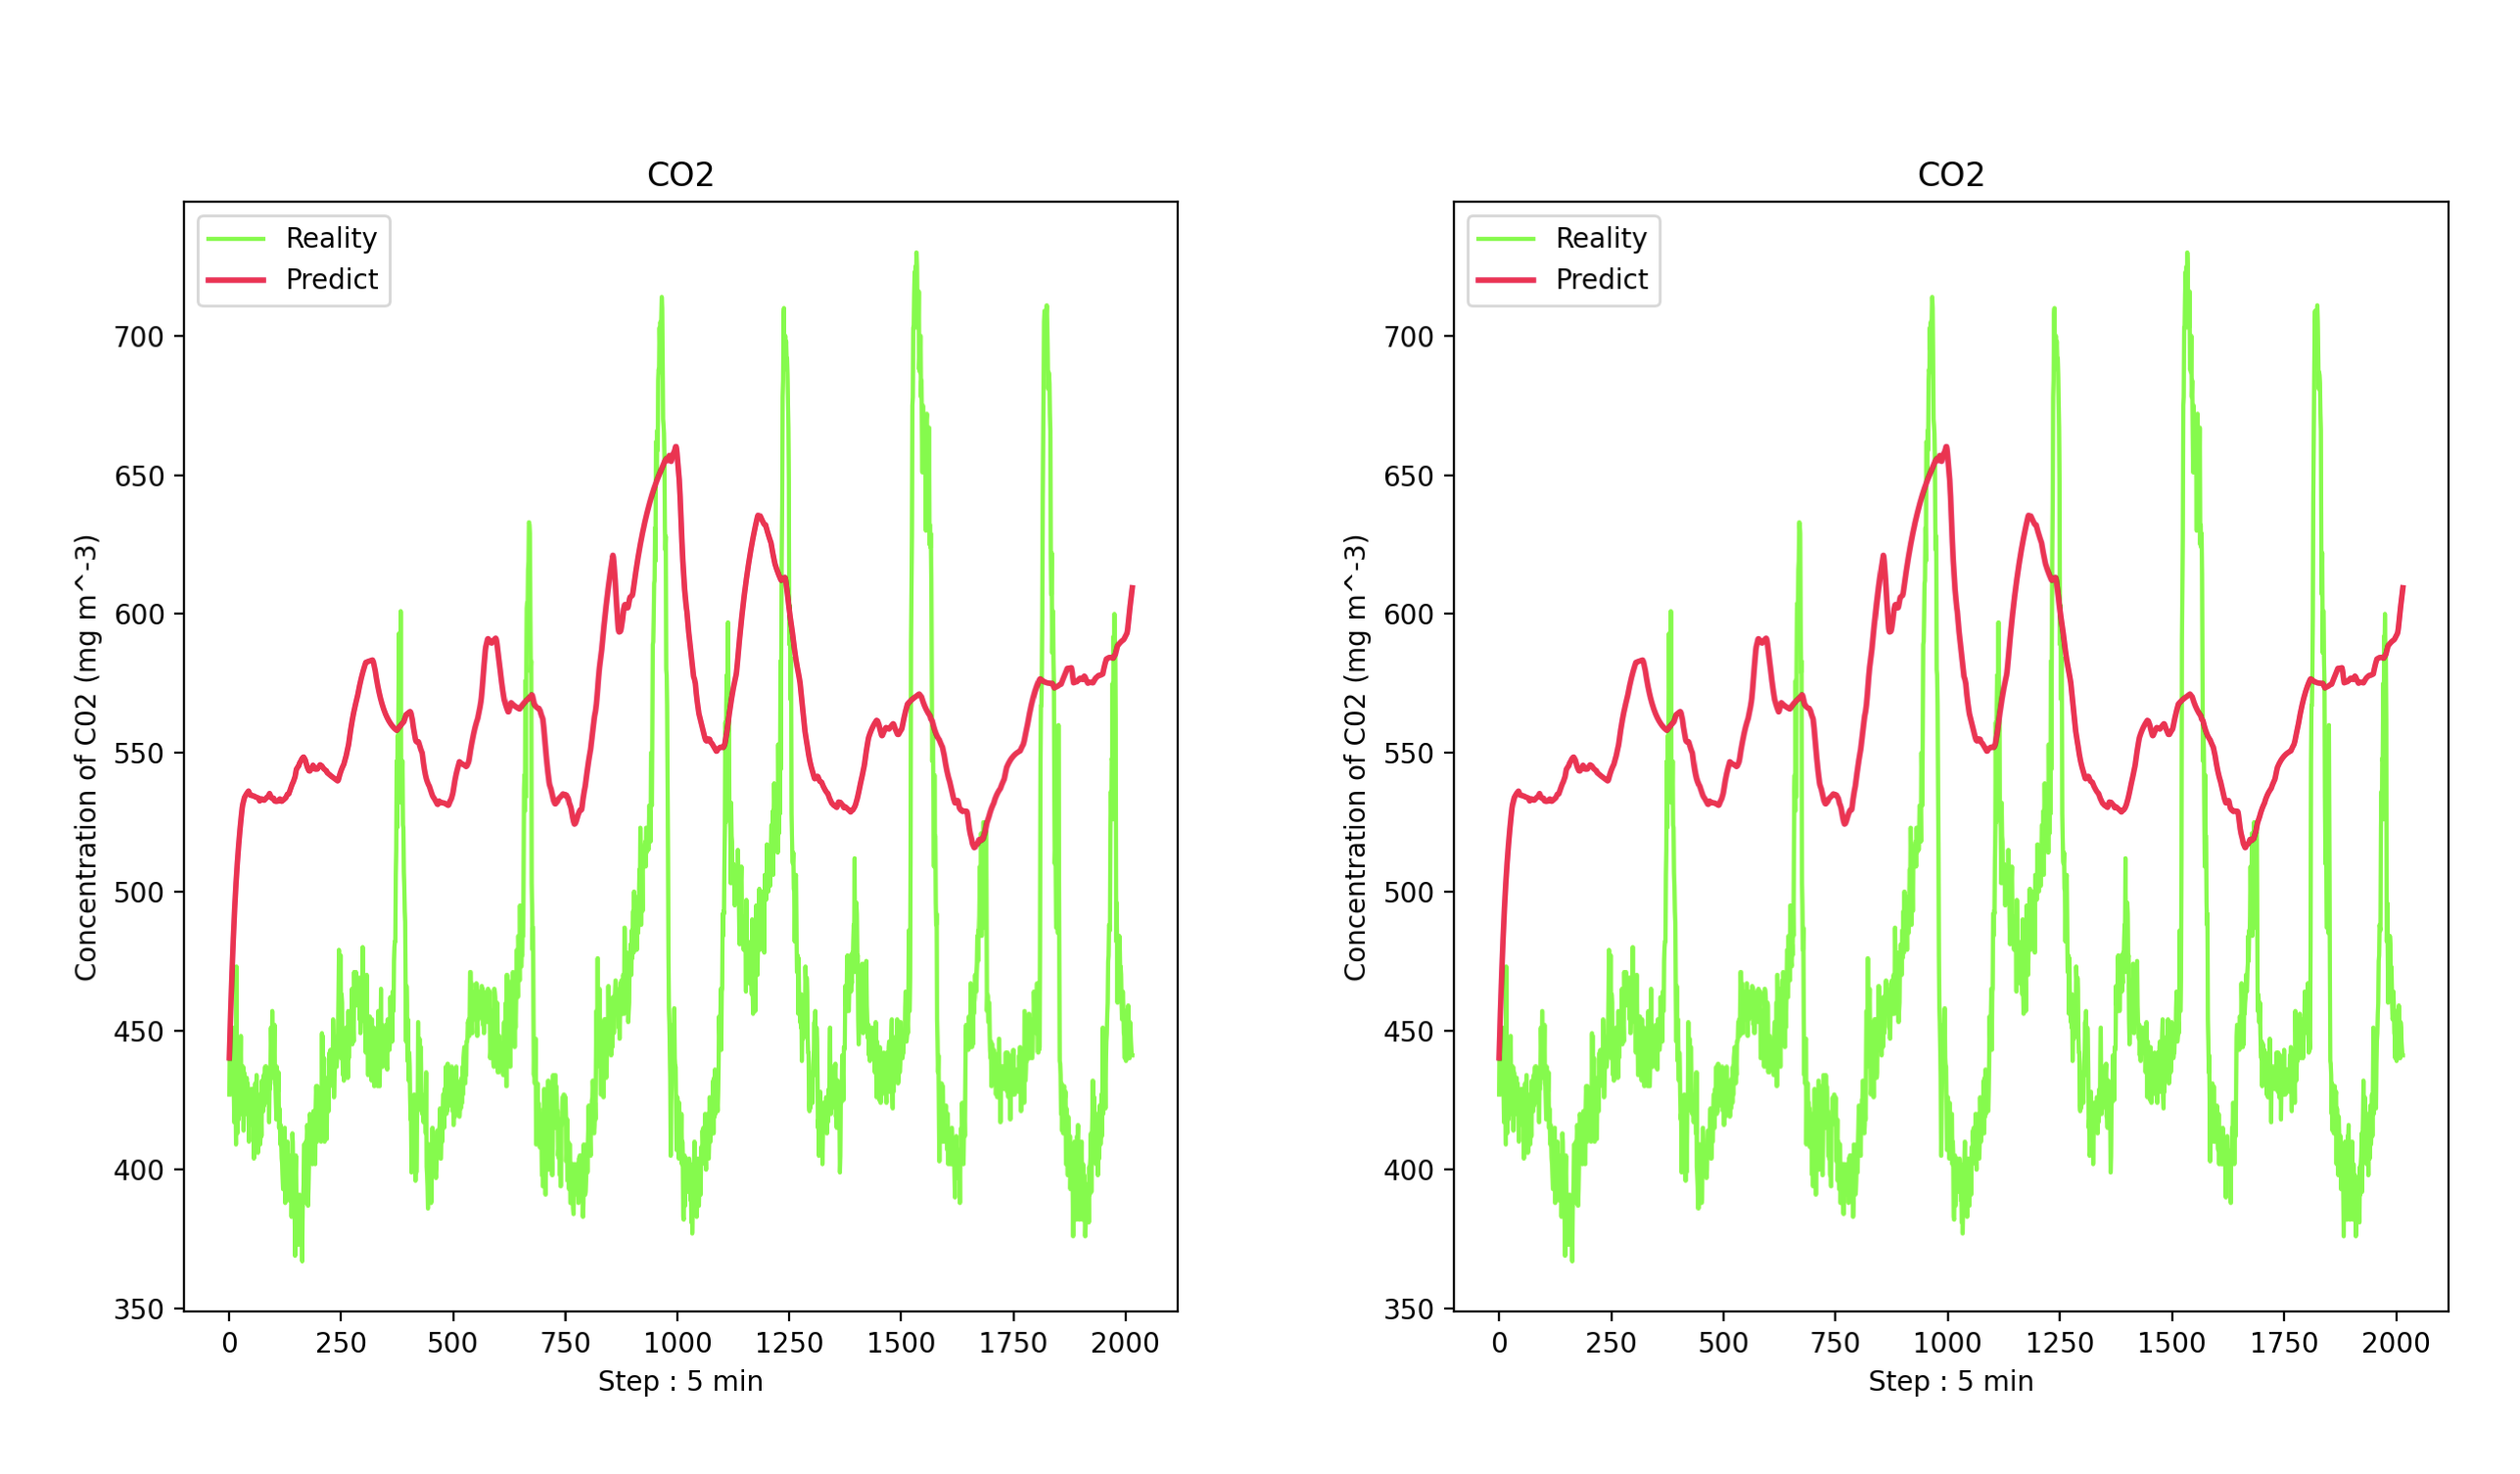
\includegraphics[width=\textwidth]{CO2_compare.png}
  \caption{\( CO_2 \) values approximation using Euler method (left) and Runge-Kutta of order 4 (right)}
\end{figure}

The Euler method and Runge-Kutta of order 4 method yield nearly identical sets of values as the approximations, even though the result obtained from the function \texttt{rk4} is slightly more accurate. The \( RMSE \) of this calculation using Euler's method is \( 117.7122\ mg\ m^{-3} \), and using Runge-Kutta's is \( 117.7114\ mg\ m^{-3} \). Even though the predictions indeed resemble the general trends in actual data, they are not close to the actual data as the difference is fairly large and is clearly noticeable in the graph. This can stem from the fact that we lack data and our model is chosen arbitrarily (arbitrary components, the climate of Texas in the data set, and the photosynthetic rate of tomatoes) despite the unawareness of the actual greenhouse model used. So, our model is not cut out for simulating the change in \( CO_2 \) concentration in the given model.

\newpage
%%%%%%%%%%%%%%%%%%%%%%%%%%%%%%%%%
\section{A dynamical system for vapor pressure}
\subsection{A vapor pressure model}
In this section, a dynamical system representing the vapor pressure in the greenhouse will be addressed.
The model was based on the following assumption:
1.\ the greenhouse air is considered to be a ``perfectly stirred tank'', meaning that there are no spatial differences in temperature, vapor pressure and the \( CO_2 \) concentration; thus all the model fluxes are described per square metre of greenhouse floor;
2.\ to describe the effect of the thermal screen on the indoor climate, the greenhouse air was divided into two compartments: one below and one above the thermal screen.

\begin{figure}[H]
  \centering
  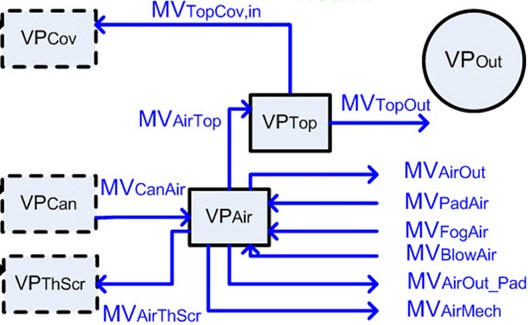
\includegraphics[width=0.6\textwidth]{VP}
  \caption{The vapor flow inside and outside a greenhouse}\label{fig:VP}
\end{figure}

The exchange in vapor pressure can be separated into three regions: \( VP_{Top} \) which is from above the screen, \( VP_{Air} \) which is from below the screen, and \( VP_{Out} \) which is from outside the greenhouse.
Their relation can be expressed as in Figure~\ref{fig:VP}.

\subsection{Dynamical systems and assumptions}
The vapor pressure of the greenhouse air \( VP_{Air} \) is described by:
\begin{multline*}
  cap_{VP_{Air}}\dot{VP_{Air}} = MV_{CanAir} + MV_{PadAir} + MV_{FogAir} + MV_{BlowAir} \\
  - MV_{AirThScr} - MV_{AirTop} - MV_{AirOut} \\
  - MV_{AirOut\_Pad} - MV_{AirMech} ~~~~ [kg\ m^{-2}\ s^{-1}]
\end{multline*}
where \( cap_{VP_{Air}} \) is the capacity of the air to store water vapor.
Vapor is exchanged between the air and surrounding elements i.e.\ the canopy \( MP_{CanAir} \), the outlet air of the pad \( MV_{PadAir} \), the fogging system \( MV_{FogAir} \), the direct air heater \( MV_{BlowAir} \), the thermal screen \( MV_{AirThScr} \), the top compartment air \( MV_{AirTop} \), the outdoor air \( MV_{AirOut} \), the outdoor air due to the air exchange caused by the pad and fan system \( MV_{AirOut\_Pad} \), and the mechanical cooling system \( MV_{AirMech} \).

The vapor pressure of the air in the top compartment \( VP_{Top} \) is described by:
\begin{multline*}
  cap_{VP_{Top}}\dot{VP_{Top}} = MV_{AirTop} - MV_{TopCov,in} - MV_{TopOut} ~~~~ [kg\ m^{-2}\ s^{-1}]
\end{multline*}
where \( cap_{VP_{Top}} \) is the capacity of the top compartment to store water vapor, \( MV_{TopCov,in} \) is the vapor exchange between the top compartment and the internal cover layer, and \( MV_{TopOut} \) is the vapor exchange between the top compartment and the outside air.

The vapor exchange coefficient between the air and an object is linearly related to the convective heat exchange coefficient between the air and the object.
Therefore, the vapor flux from the air to an object by condensation is described by:
\begin{align}
  \label{eq:vapor_conden}
  MV_{12} = \begin{cases}
    0                                       & \text{if~} VP_1 < VP_2 \\
    6.4 \cdot 10^{-9} HEC_{12}(VP_1 - VP_2) & \text{if~} VP_1 > VP_2 \\
  \end{cases}
\end{align}
where \( MV_{12} \) (\( kg\ m^{-2}\ s^{-1} \)) is the vapor flux from air of location 1 to object 2, \( 6.4 \cdot 10^{-9} \) is the conversion factor relating the heat exchange coefficient (\( W\ m^{-2}\ K^{-1} \)) to the vapor exchange coefficient (\( kg\ m^{-2}\ s^{-1}\ Pa^{-1} \)), \( HEC_{12} \) (\( W\ m^{-2}\ K^{-1} \)) is the heat exchange coefficient between the air of location 1 to object 2 and \( VP_1 \) (\( Pa \)) is the vapor pressure of the air of location 1 and \( VP_2 \) is the saturated vapor pressure of object 2 at its temperature.

Because this model should consist of only differentiable functions, equation~\eqref{eq:vapor_conden} was smoothed to:
\begin{align}
  MV_{12} = \frac{1}{1 + \exp \left(s_{MV_{12}} (VP_1 - VP_2)\right)} \cdot 6.4 \cdot 10^{-9} HEC_{12} (VP_1 - VP_2)
\end{align}
where \( s_{MV_{12}} \) (\( - \)) is the slope of the differentiable switch function for vapor pressure differences.

% AirThScr
The vapor flux from the greenhouse air compartment to the thermal screen and the vapor flux from the top compartment to the interval cover layer are described analogously to equation~\eqref{eq:vapor_conden}:
\begin{align}
  MV_{AirThScr}  & = \begin{cases}
    0                                                       & \text{if~} VP_{Air} < VP_{ThScr} \\
    6.4 \cdot 10^{-9} HEC_{AirThScr}(VP_{Air} - VP_{ThScr}) & \text{if~} VP_{Air} > VP_{ThScr} \\
  \end{cases} \\
  % TopCov,in
  MV_{TopCov,in} & = \begin{cases}
    0                                                         & \text{if~} VP_{Top} < VP_{Cov,in} \\
    6.4 \cdot 10^{-9} HEC_{TopCov,in}(VP_{Top} - VP_{Cov,in}) & \text{if~} VP_{Top} > VP_{Cov,in} \\
  \end{cases}
\end{align}
whereby their associated heat change coefficients are:
\begin{align}
  HEC_{AirThScr}  & = 1.7 U_{ThScr} |T_{Air} - T_{ThScr}|^{0.33}                        \\
  HEC_{TopCov,in} & = {c_{HECin} (T_{Top} - T_{Cov,in})}^{0.33} \frac{A_{Cov}}{A_{Flr}}
\end{align}
with \( U_{ThScr} \in [0,1] \) representing the percentage of places that are covered by the thermal screen, \( T_X \) (\( \celsius \)) is the temperature at location \( X \), \( c_{HECin} \) (\( W\ m^{-2}\ K^{-2} \)) is the convective heat exchange parameter between cover and outdoor air depending on the greenhouse shape, \( A_{Cov} \) (\( m^2 \)) is the surface of the cover including the side-walls, and \( A_{Flr} \) (\( m^2 \)) is the surface of the greenhouse floor.

The general form of a vapor flux accompanying an air flux is described by:
\begin{align}
  \label{eq:vapor_air}
  MV_{12} = \frac{M_{Water}}{R} f_{12} \left(\frac{VP_1}{T_1 + 273.15} - \frac{VP_2}{T_2 + 273.15}\right)
\end{align}
where \( MV_{12} \) (\( kg\ m^{-2}\ s^{-1} \)) is the vapor flux from location 1 to location 2, \( f_{12} \) (\( m^3\ m^{-2}\ s^{-1} \)) is the air flux from location 1 to location 2, \( T_1 \) and \( T_2 \) (\( \celsius \)) are the temperature at location 1 and 2 respectively.

% AirTop
The vapor fluxes from the air compartment to the top compartment, the air compartment to the outdoor air, and the top compartment to the outdoor air are described analogously to equation~\eqref{eq:vapor_air}:
\begin{align}
  MV_{AirTop} & = \frac{M_{Water}}{R} f_{ThScr} \left(\frac{VP_{Air}}{T_{Air} + 273.15} - \frac{VP_{Top}}{T_{Top} + 273.15}\right)                       \\
  % AirOut
  MV_{AirOut} & = \frac{M_{Water}}{R} (f_{VentSide} + f_{VentForced}) \left(\frac{VP_{Air}}{T_{Air} + 273.15} - \frac{VP_{Out}}{T_{Out} + 273.15}\right) \\
  % TopOut
  MV_{TopOut} & = \frac{M_{Water}}{R} f_{VentRoof} \left(\frac{VP_{Top}}{T_{Top} + 273.15} - \frac{VP_{Out}}{T_{Out} + 273.15}\right)
\end{align}

% CanAir
The canopy transpiration is described by:
\begin{align}
  MV_{CanAir} = VEC_{CanAir}(VP_{Can} - VP_{Air})
\end{align}
where \( VEC_{CanAir} \) (\( kg\ Pa\ s^{-1} \)) is the vapor exchange coefficient between the canopy and air, \( VP_{Can} \) is the saturated vapor pressure at canopy temperature.

According to Stanghellini (1987), the vapor transfer coefficient of the canopy transpiration can be calculated by:
\begin{align}
  VEC_{CanAir} = \frac{2 \rho_{Air} c_{p,Air}LAI}{\Delta H \gamma (r_b + r_s)}
\end{align}
where \( \rho_{Air} \) (\( kg\ m^{-3} \)) is the density of the greenhouse air, \( c_{p,Air} \) (\( J\ K^{-1}\ kg^{-1} \)) is the specific heat capacity of the greenhouse air, \( LAI \) (\( m^2\ m^{-2} \)) is the leaf area index, \( \Delta H \) (\( J\ kg^{-1} \)) is the latent heat of evaporation of water, \( \gamma \) (\( Pa\ K^{-1} \)) is the psychometric constant, \( r_b \) (\( s\ m^{-1} \)) is the boundary layer resistance of the canopy for vapor transport and \( r_s \) (\( s\ m^{-1} \)) is the stomatal resistance of the canopy for vapor transport.

The boundary layer resistance for vapor transport depends on the wind speed in the greenhouse and the temperature difference between the canopy and surrounding air\cite{stanghellini1987transpiration}.
However, the wind speed in the greenhouse is not measured nor simulated and therefore a constant boundary layer resistance was used.
The stomatal resistance of the canopy is described by a simplification of the stomatal resistance model of Stanghellini (1987):
\begin{align}
  r_s = r_{s,\min} \cdot rf(R_{Can}) \cdot rf(CO_{2Air\_ppm}) \cdot rf(VP_{Can} - VP_{Air})
\end{align}
where \( r_{s,\min} \) (\( s\ m^{-1} \)) is the minimum canopy resistance and \( rf \) is the resistance factor for high radiation levels, high \( CO_2 \) levels and large vapor pressure differences.
The resistance factors are described according to Stangellini (1987):
\begin{equation}
  \begin{split}
    rf(R_{Can}) & = \frac{R_{Can} + c_{evap1}}{R_{Can} + c_{evap2}} \\
    rf(CO_{2Air}) & = 1 + {c_{evap3} (\eta_{mg\_ppm} CO_{2Air} - 200)}^2 \\
    rf(VP_{Can} - VP_{Air}) & = 1 + {c_{evap4} (VP_{Can} - VP_{Air})}^2
  \end{split}
\end{equation}

where \( R_{Can} \) (\( W\ m^{-2} \)) is the global radiation above the canopy, \( c_{evap1} \) (\( W\ m^{-2} \)), \( c_{evap2} \) (\( W\ m^{-2} \)), \( c_{evap3} \) (\( ppm^{-2} \)), \( c_{evap4} \) (\( Pa^{-2} \)) are empirically determined parameters and \( \eta_{mg\_ppm} \) (\( ppm\ mg^{-1}\ m^3 \)) is the conversion factor from \( mg\ m^{-3}\ CO_2 \) to \( ppm \).
Stanghellini limited the resistance factor for high \( CO_2 \) levels to 1.5 and the resistance factor for large vapor pressure differences to 5.8 and determined the transpiration variables \( c_{evap3} \) and \( c_{evap4} \) for day time and night time.
The values of the transpiration parameters \( c_{evap3} \) and \( c_{evap4} \) differed between the night period and day period which means that the accompanying equations are not differentiable at sunrise and sunset. Therefore the parameters \( c_{evap3} \) and \( c_{evap4} \) were smoothed using the differentiable switch function:
\begin{align}
  S_{r_s} = \frac{1}{1 + \exp \left(s_{r_s} (R_{Can} - R_{Can\_SP})\right)}
\end{align}
where \( S_{r_s} \) (\( - \)) is the value of the differentiable switch, \( s_{r_s} \) (\( m\ W^{-2} \)) is the slope of the differentiable switch for the stomatal resistance model and \( R_{Can\_SP} \) (\( W\ m^{-2} \)) is the radiation value above the canopy to define sunrise and sunset.
Using the differential switch, the smoothed transpiration parameters were described by:
\begin{align}
  c_{evap3} & = c_{evap3}^{day} (1 - S_{r_s}) + c_{evap3}^{night} S_{r_s} \\
  c_{evap4} & = c_{evap4}^{day} (1 - S_{r_s}) + c_{evap4}^{night} S_{r_s}
\end{align}

% BlowAir
The vapor flux from the heat blower to the greenhouse air is proportional to the heat flux:
\begin{align}
  MV_{BlowAir} = \eta_{HeatVap} H_{BlowAir}
\end{align}
where \( \eta_{HeatVap} \) (\( kg\{vapor\}\ J^{-1} \)) is the amount of vapor which is released when 1 Joule of sensible energy is produced by the direct air heater.

% PadAir
The vapor flux from the pad and fan to the greenhouse air is described by:
\begin{align}
  MV_{PadAir} = \rho_{Air} f_{Pad} (\eta_{Pad} (x_{Pad} - x_{Out}) + x_{Out})
\end{align}
where \( f_{Pad} \) (\( m^3\ m^{-2}\ s^{-1} \)) is the ventilation flux due to the pad and fan system, \( \eta_{Pad} \) (\( - \)) is the efficiency of the pad and fan system, \( x_{Pad} \) (\( kg\{water\} kg^{-1}\{air\} \)) is the water vapor content of the pad and \( x_{Out} \) (\( kg\{water\} kg^{-1}\{air\} \)) is the water vapor content of the outdoor air.

The ventilation flux due to the pad and fan system is described by:
\begin{align}
  f_{Pad} = \frac{U_{Pad} \phi_{Pad}}{A_{Flr}}
\end{align}
where \( U_{Pad} \) (\( - \)) is the control valve of the pad and fan system and \( \phi_{Pad} \) (\( m^3\ s^{-1} \)) is the capacity of the air flux through the pad.

% AirOut_Pad
The vapor flux from the greenhouse air to the outside air when using the pad and fan system is described by:
\begin{align}
  MV_{AirOut\_Pad} = f_{Pad} \frac{M_{Water}}{R} \left(\frac{VP_{Air}}{T_{Air} + 273.15}\right)
\end{align}

% AirMech
The vapor flux from the greenhouse air to the surface of mechanical cooling system is described analogously to equation~\eqref{eq:vapor_conden}:
\begin{align}
  MV_{AirMech} = \begin{cases}
    0                                                     & \text{if~} VP_{Air} < VP_{Mech} \\
    6.4 \cdot 10^{-9} HEC_{AirMech}(VP_{Air} - VP_{Mech}) & \text{if~} VP_{Air} > VP_{Mech} \\
  \end{cases}
\end{align}
with \( HEC_{AirMech} \) is the heat exchange coefficient between the greenhouse air and the surface of the mechanical cooling unit:
\begin{align}
  HEC_{AirMech} = \frac{U_{MechCool} COP_{MechCool} P_{MechCool} / A_{Flr}}{T_{Air} - T_{MechCool} + 6.4 \cdot 10^{-9} \Delta H(VP_{Air} - VP_{MechCool})}
\end{align}
where \( U_{MechCool} \) (\( - \)) is the control valve of the mechanical cooling mechanism, \( COP_{MechCool} \) (\( - \)) is the coefficient of performance of the mechanical cooling system and \( P_{MechCool} \) is the electrical capacity of the mechanical cooling system, \( T_{MechCool} \) (\( \celsius \)) is the temperature of the cooling surface, and \( VP_{MechCool} \) (\( Pa \)) is the saturated vapor pressure of the mechanical cooling mechanism.

% FogAir
The latent heat flux from the greenhouse air depends on the vapor flux from the fogging system to the greenhouse air which is described by:
\begin{align}
  MV_{FogAir} = \frac{U_{Fog} \phi_{Fog}}{A_{Flr}}
\end{align}
where \( U_{Fog} \) (\( - \)) is the control valve of the fogging system and \( \phi_{Fog} \) (\( kg\{water\}\ s^{-1} \)) is the capacity of the fogging system.

\newpage
\subsection{Implementing the programs}
To calculate \( \dot{VP_{Air}} \) and \( \dot{VP_{Top}} \), we use the following \( dx \) function.
Each \( MV \) of the formula will be given and explained further below.
\begin{mdframed}[leftline=false,rightline=false,backgroundcolor=magenta!10,nobreak=true]
  \begin{minted}[linenos,breaklines,breaksymbolleft=,obeytabs=true,tabsize=2]{Python}
def dx_VP(self, t, VP_Air, VP_Top):
    # Update environment variable at time t (s)
    self.update(data_Tair[int(t / 300)],
                data_Tout[int(t / 300)],
                wind_speed[int(t / 300)])

    self.VP_Air = VP_Air
    self.VP_Top = VP_Top

    cap_VPAir = self.cap_VPAir()
    cap_VPTop = self.cap_VPTop()
    MV_CanAir = self.MV_CanAir()
    MV_PadAir = self.MV_PadAir()
    MV_FogAir = self.MV_FogAir()
    MV_BlowAir = self.MV_BlowAir()
    MV_AirThScr = self.MV_AirThScr()
    MV_AirTop = self.MV_AirTop()
    MV_AirOut = self.MV_AirOut()
    MV_AirOutPad = self.MV_AirOutPad()
    MV_AirMech = self.MV_AirMech()
    MV_TopCovin = self.MV_TopCovin()
    MV_TopOut = self.MV_TopOut()
    return ((MV_CanAir + MV_PadAir + MV_FogAir + MV_BlowAir - MV_AirThScr - MV_AirTop - MV_AirOut - MV_AirOutPad - MV_AirMech) / cap_VPAir,
            (MV_AirTop - MV_TopCovin - MV_TopOut) / cap_VPTop)
  \end{minted}
\end{mdframed}

The following instructions are called multiple times.
They have been gathered here for improved readability.
\begin{mdframed}[leftline=false,rightline=false,backgroundcolor=magenta!10,nobreak=true]
  \begin{minted}[linenos,breaklines,breaksymbolleft=,obeytabs=true,tabsize=2]{Python}
def vapour_flux(self, f, VP_from, T_from, VP_to, T_to):
    return self.Constant.M_WATER / self.Constant.M_GAS * f * (VP_from / (T_from + 273.15) - VP_to / (T_to + 273.15))
  \end{minted}
\end{mdframed}
\begin{mdframed}[leftline=false,rightline=false,backgroundcolor=magenta!10,nobreak=true]
  \begin{minted}[linenos,breaklines,breaksymbolleft=,obeytabs=true,tabsize=2]{Python}
def air_density(self):
    return self.Constant.DENSITY_AIR0 * math.exp(
        self.Constant.GRAVITY * self.Constant.M_AIR * self.Coefficients.Construction.elevation_height / (
            293.15 * self.Constant.M_GAS))
  \end{minted}
\end{mdframed}
\begin{mdframed}[leftline=false,rightline=false,backgroundcolor=magenta!10,nobreak=true]
  \begin{minted}[linenos,breaklines,breaksymbolleft=,obeytabs=true,tabsize=2]{Python}
def saturation_vapor_pressure(temp):
    # Calculation based on
    return 610.78 * math.exp(temp / (temp + 238.3) * 17.2694)
  \end{minted}
\end{mdframed}
\begin{mdframed}[leftline=false,rightline=false,backgroundcolor=magenta!10,nobreak=true]
  \begin{minted}[linenos,breaklines,breaksymbolleft=,obeytabs=true,tabsize=2]{Python}
def eta_InsScr_(self):
    eta_InsScr = self.eta_InsScr
    return eta_InsScr * (1 - eta_InsScr)
  \end{minted}
\end{mdframed}


The vapor fluxes have been implemented as follows:

% AirThScr
\( MV_{AirThScr} \):
\begin{mdframed}[leftline=false,rightline=false,backgroundcolor=magenta!10,nobreak=true]
  \begin{minted}[linenos,breaklines,breaksymbolleft=,obeytabs=true,tabsize=2]{Python}
def MV_AirThScr(self):
    # HEC_AirThScr
    U_ThScr = self.Assuming.U_ThScr
    T_ThScr = self.ClimateStates.T_ThScr
    T_Air = self.ClimateStates.T_Air
    HEC_AirThScr = 1.7 * U_ThScr * abs(T_Air - T_ThScr) ** 0.33


    VP_Air = self.ClimateStates.VP_Air
    VP_ThScr = self.saturation_vapor_pressure(T_ThScr)
    if VP_Air < VP_ThScr:
        return 0
    else:
        return 6.4E-9 * HEC_AirThScr * (VP_Air - VP_ThScr)
  \end{minted}
\end{mdframed}

% TopCov,in
\( MV_{TopCov,in} \):
\begin{mdframed}[leftline=false,rightline=false,backgroundcolor=magenta!10,nobreak=true]
  \begin{minted}[linenos,breaklines,breaksymbolleft=,obeytabs=true,tabsize=2]{Python}
def MV_TopCovin(self):
    # =============== HEC_TopCovin
    c_HECin = self.Coefficients.Construction.c_HECin
    T_Top = self.ClimateStates.T_Top
    T_Covin = self.ClimateStates.T_Cov_in
    A_Cov = self.Coefficients.Construction.cover_area
    A_Flr = self.Coefficients.Construction.floor_area
    HEC_TopCovin = c_HECin * (T_Top - T_Covin) ** (1/3) * A_Cov / A_Flr
    # ===============

    VP_Top = self.ClimateStates.VP_Top
    VP_Covin = self.saturation_vapor_pressure(T_Covin)
    if VP_Top < VP_Covin:
        return 0
    else:
        return 6.4E-9 * HEC_TopCovin * (VP_Top - VP_Covin)
  \end{minted}
\end{mdframed}

% AirTop
\( MV_{AirTop} \):
\begin{mdframed}[leftline=false,rightline=false,backgroundcolor=magenta!10,nobreak=true]
  \begin{minted}[linenos,breaklines,breaksymbolleft=,obeytabs=true,tabsize=2]{Python}
def MV_AirTop(self):
    f_ThScr = self.f_ThScr()
    VP_Air = self.ClimateStates.VP_Air
    T_Air = self.ClimateStates.T_Air
    VP_Top = self.ClimateStates.VP_Top
    T_Top = self.ClimateStates.T_Top
    return self.vapour_flux(f_ThScr, VP_Air, T_Air, VP_Top, T_Top)
  \end{minted}
\end{mdframed}
\begin{mdframed}[leftline=false,rightline=false,backgroundcolor=magenta!10,nobreak=true]
  \begin{minted}[linenos,breaklines,breaksymbolleft=,obeytabs=true,tabsize=2]{Python}
def f_ThScr(self):
    # Equation 8.41
    U_ThScr = self.U_ThScr
    K_ThScr = self.K_ThScr
    T_Air = self.T_Air
    T_Out = self.T_Out
    p_Air = self.air_density()
    pressure = 101325 * (1 - 2.5577e-5 * self.elevation_height) ** 5.25588
    p_Out = M_AIR * pressure / ((self.T_Top + 273.15) * M_GAS)
    p_Mean = (p_Air + p_Out) / 2

    return U_ThScr * K_ThScr * abs(T_Air - T_Out) ** 0.66 + (1 - U_ThScr) / p_Mean * math.sqrt(
        0.5 * p_Mean * (1 - U_ThScr) * GRAVITY * abs(p_Air - p_Out))
  \end{minted}
\end{mdframed}

% AirOut
\( MV_{AirOut} \):
This model assumes that forced ventilation is not used, thus some functions have been deducted.
\begin{mdframed}[leftline=false,rightline=false,backgroundcolor=magenta!10,nobreak=true]
  \begin{minted}[linenos,breaklines,breaksymbolleft=,obeytabs=true,tabsize=2]{Python}
def MV_AirOut(self):
    f_VentSide = self.f_VentSide()
    f_VentForced = self.f_VentForced()
    f_AirOut = f_VentSide + f_VentForced
    VP_Air = self.ClimateStates.VP_Air
    T_Air = self.ClimateStates.T_Air
    VP_Out = self.Weather.VP_Out
    T_Out = self.Weather.T_Out
    return self.vapour_flux(f_AirOut, VP_Air, T_Air, VP_Out, T_Out)
  \end{minted}
\end{mdframed}
\begin{mdframed}[leftline=false,rightline=false,backgroundcolor=magenta!10,nobreak=true]
  \begin{minted}[linenos,breaklines,breaksymbolleft=,obeytabs=true,tabsize=2]{Python}
def f_VentSide(self):
    eta_Side = 0
    eta_Roof = 1
    eta_InsScr = self.eta_InsScr()
    d2_f_VentSide = self.d2_f_VentSide()
    d2_f_VentRoofSide = self.d2_f_VentRoofSide()
    f_leakage = self.f_leakage()
    U_ThScr = self.Assuming.U_ThScr

    if eta_Side >= self.Constant.ETA_ROOF_THR:
        return eta_InsScr * d2_f_VentSide + 0.5 * f_leakage
    else:
        return eta_InsScr * (
            U_ThScr * d2_f_VentSide + (1 - U_ThScr) * d2_f_VentRoofSide * eta_Side) + 0.5 * f_leakage
  \end{minted}
\end{mdframed}
\begin{mdframed}[leftline=false,rightline=false,backgroundcolor=magenta!10,nobreak=true]
  \begin{minted}[linenos,breaklines,breaksymbolleft=,obeytabs=true,tabsize=2]{Python}
def f_VentForced(self):
    return 0
  \end{minted}
\end{mdframed}
\begin{mdframed}[leftline=false,rightline=false,backgroundcolor=magenta!10,nobreak=true]
  \begin{minted}[linenos,breaklines,breaksymbolleft=,obeytabs=true,tabsize=2]{Python}
def d2_f_VentRoofSide(self):
    U_Roof = self.U_Roof
    U_Side = self.U_Side
    A_Roof = self.roof_ventilation_area
    A_Side = self.side_ventilation_area
    A_Flr = self.floor_area
    h_SideRoof = self.h_SideRoof
    C_d = self.C_d
    C_w = self.C_w
    T_Air = self.T_Air
    T_Out = self.T_Out
    T_Mean = (T_Air + T_Out) / 2
    v_Wind = self.v_Wind
    AU_Roof = A_Roof * U_Roof
    AU_Side = A_Side * U_Side
    return C_d / A_Flr * math.sqrt((AU_Roof * AU_Side / math.sqrt(AU_Roof ** 2 + AU_Side ** 2)) ** 2 * (
        2 * GRAVITY * h_SideRoof * (T_Air - T_Out) / (T_Mean + 273.15)) + 0.25 * (
        AU_Roof + AU_Side) ** 2 * C_w * v_Wind ** 2)
  \end{minted}
\end{mdframed}
\begin{mdframed}[leftline=false,rightline=false,backgroundcolor=magenta!10,nobreak=true]
  \begin{minted}[linenos,breaklines,breaksymbolleft=,obeytabs=true,tabsize=2]{Python}
def f_leakage(self):
    c_leakage = self.Coefficients.Ventilation.c_leakage
    v_Wind = self.Weather.v_Wind
    return c_leakage * max(0.25, v_Wind)
  \end{minted}
\end{mdframed}

% TopOut
\( MV_{TopOut} \):
\begin{mdframed}[leftline=false,rightline=false,backgroundcolor=magenta!10,nobreak=true]
  \begin{minted}[linenos,breaklines,breaksymbolleft=,obeytabs=true,tabsize=2]{Python}
def MV_TopOut(self):
    f_VentRoof = self.f_VentRoof()
    VP_Top = self.ClimateStates.VP_Top
    T_Top = self.ClimateStates.T_Top
    VP_Out = self.Weather.VP_Out
    T_Out = self.Weather.T_Out
    return self.vapour_flux(f_VentRoof, VP_Top, T_Top, VP_Out, T_Out)
  \end{minted}
\end{mdframed}
\begin{mdframed}[leftline=false,rightline=false,backgroundcolor=magenta!10,nobreak=true]
  \begin{minted}[linenos,breaklines,breaksymbolleft=,obeytabs=true,tabsize=2]{Python}
def f_VentRoof(self):
    eta_Roof = 1
    eta_InsScr = self.eta_InsScr()
    d2_f_VentRoof = self.d2_f_VentRoof()
    d2_f_VentRoofSide = self.d2_f_VentRoofSide()
    f_leakage = self.f_leakage()
    U_ThScr = self.Assuming.U_ThScr
    if eta_Roof >= self.Constant.ETA_ROOF_THR:
        return eta_InsScr * d2_f_VentRoof + 0.5 * f_leakage
    else:
        return eta_InsScr * (
            U_ThScr * d2_f_VentRoof + (1 - U_ThScr) * d2_f_VentRoofSide * eta_Roof) + 0.5 * f_leakage
  \end{minted}
\end{mdframed}

% CanAir
\( MV_{CanAir} \):
\begin{mdframed}[leftline=false,rightline=false,backgroundcolor=magenta!10,nobreak=true]
  \begin{minted}[linenos,breaklines,breaksymbolleft=,obeytabs=true,tabsize=2]{Python}
def MV_CanAir(self):
    # ================= VEC Can Air
    p_Air = self.air_density()
    LAI = self.LAI
    VEC_CanAir = 2 * p_Air * C_PAIR * LAI / (
        EVAPORATION_LATENT_HEAT * GAMMA * (
            BOUNDARY_LAYER_RESISTANCE + MIN_CANOPY_TRANSPIRATION_RESISTANCE))
    # =================

    VP_Air = self.VP_Air
    VP_Can = self.saturation_vapor_pressure(self.T_Can)
    return VEC_CanAir * (VP_Can - VP_Air)
  \end{minted}
\end{mdframed}

% BlowAir
\( MV_{BlowAir} \):
\begin{mdframed}[leftline=false,rightline=false,backgroundcolor=magenta!10,nobreak=true]
  \begin{minted}[linenos,breaklines,breaksymbolleft=,obeytabs=true,tabsize=2]{Python}
def MV_BlowAir(self):
    U_Blow = self.U_Blow
    P_Plow = self.P_Blow
    A_Flr = self.floor_area
    return ETA_HEATVAP * U_Blow * P_Plow / A_Flr
  \end{minted}
\end{mdframed}

% PadAir
\( MV_{PadAir} \):
This system assumes that ventilation via pad and fan system is not used.
\begin{mdframed}[leftline=false,rightline=false,backgroundcolor=magenta!10,nobreak=true]
  \begin{minted}[linenos,breaklines,breaksymbolleft=,obeytabs=true,tabsize=2]{Python}
def MV_PadAir(self):
    return 0
  \end{minted}
\end{mdframed}

% AirOut_Pad
\( MV_{AirOut\_Pad} \):
\begin{mdframed}[leftline=false,rightline=false,backgroundcolor=magenta!10,nobreak=true]
  \begin{minted}[linenos,breaklines,breaksymbolleft=,obeytabs=true,tabsize=2]{Python}
def MV_AirOutPad(self):
    U_Pad = self.U_Pad
    phi_Pad = self.phi_Pad
    A_Flr = self.floor_area
    VP_Air = self.VP_Air
    T_Air = self.T_Air
    return U_Pad * phi_Pad / A_Flr * M_WATER / M_GAS * VP_Air / (T_Air + 273.15)
  \end{minted}
\end{mdframed}

% AirMech
\( MV_{AirMech} \):
This model assumes that mechanical cooling is not used.
\begin{mdframed}[leftline=false,rightline=false,backgroundcolor=magenta!10,nobreak=true]
  \begin{minted}[linenos,breaklines,breaksymbolleft=,obeytabs=true,tabsize=2]{Python}
def MV_AirMech(self):
    return 0
  \end{minted}
\end{mdframed}

% FogAir
\( MV_{FogAir} \):
\begin{mdframed}[leftline=false,rightline=false,backgroundcolor=magenta!10,nobreak=true]
  \begin{minted}[linenos,breaklines,breaksymbolleft=,obeytabs=true,tabsize=2]{Python}
def MV_FogAir(self):
    U_Fog = self.U_Fog
    phi_Fog = self.phi_Fog
    A_Flr = self.floor_area
    return U_Fog * phi_Fog / A_Flr
  \end{minted}
\end{mdframed}

\subsection{Testing the programs}
The data used in this model is based on the climate of Texas in United States and the photosynthesis model is based on tomatoes.
We will consider the first step where the values of the initial state are: \( VP_{Air} = VP_{Top} = 2300 \).
\begin{itemize}
  \item \textbf{Function \texttt{MV\_AirThScr()} is equivalent to equation:}
        \begin{align*}
          MV_{AirThScr} & = \begin{cases}
            0                                                       & \text{if~} VP_{Air} < VP_{ThScr} \\
            6.4 \cdot 10^{-9} HEC_{AirThScr}(VP_{Air} - VP_{ThScr}) & \text{if~} VP_{Air} > VP_{ThScr} \\
          \end{cases}
        \end{align*}
        where
        \begin{align*}
          HEC_{AirThScr} & = 1.7 U_{ThScr} |T_{Air} - T_{ThScr}|^{0.33}
        \end{align*}

        \begin{table}[H]
          \centering
          \begin{tabular}{@{}lS[table-format=4.17]@{}}
            \toprule
            \textbf{Variable}  & \textbf{Value}     \\
            \midrule
            \( U_{ThScr} \)      & 0.863              \\
            \( T_{Air} \)        & 19.8999999966472   \\
            \( T_{ThScr} \)      & 20.8999999966472   \\
            \( HEC_{AirThScr} \) & 1.4670999999999998 \\
            \( VP_{Air} \)       & 2300               \\
            \( VP_{ThScr} \)     & 2458.2757172240395 \\
            \bottomrule
          \end{tabular}
        \end{table}

  \item[-] Result of this equation: \( MV_{AirThScr} = 0 \)

  \item \textbf{Function \texttt{MV\_TopCovin()} is equivalent to equation:}
        \begin{align*}
          MV_{TopCov,in} & = \begin{cases}
            0                                                         & \text{if~} VP_{Top} < VP_{Cov,in} \\
            6.4 \cdot 10^{-9} HEC_{TopCov,in}(VP_{Top} - VP_{Cov,in}) & \text{if~} VP_{Top} > VP_{Cov,in} \\
          \end{cases}
        \end{align*}
        where
        \begin{align*}
          HEC_{TopCov,in} & = {c_{HECin} (T_{Top} - T_{Cov,in})}^{0.33} \frac{A_{Cov}}{A_{Flr}}
        \end{align*}

        \begin{table}[H]
          \centering
          \begin{tabular}{@{}lS[table-format=4.17]@{}}
            \toprule
            \textbf{Variable}  & \textbf{Value}     \\
            \midrule
            \( c_{HECin} \)      & 1.86               \\
            \( T_{Top} \)        & 21.3999999966472   \\
            \( T_{Covin} \)      & 20.8999999966472   \\
            \( A_{Cov} \)        & 80000              \\
            \( A_{Flr} \)        & 70000              \\
            \( HEC_{TopCovin} \) & 1.7266165225401122 \\
            \( VP_{Top} \)       & 2300               \\
            \( VP_{Covin} \)     & 2458.2757172240395 \\
            \bottomrule
          \end{tabular}
        \end{table}

  \item[-] Result of this equation: \( MV_{TopCov,in} = 0 \)

  \item \textbf{Function \texttt{MV\_AirTop()} is equivalent to equation:}
        \begin{align*}
          MV_{AirTop}  = \frac{M_{Water}}{R} f_{ThScr} (\frac{VP_{Air}}{T_{Air} + 273.15} - \frac{VP_{Top}}{T_{Top} + 273.15})
        \end{align*}

        \begin{table}[H]
          \centering
          \begin{tabular}{@{}lS[table-format=4.17]@{}}
            \toprule
            \textbf{Variable} & \textbf{Value}      \\
            \midrule
            \( M_{Water} \)     & 18.01528            \\
            \( R \)             & 8314                \\
            \( f_{ThScr} \)     & 0.06867093888863662 \\
            \( VP_{Air} \)      & 2300                \\
            \( T_{Air} \)       & 19.8999999966472    \\
            \( VP_{Top} \)      & 2300                \\
            \( T_{Top} \)       & 21.3999999966472    \\
            \bottomrule
          \end{tabular}
        \end{table}

  \item [-] Function \hyperref[fThScr]{\underline{\( f\_ThScr() \)}} is already described in Chapter 3, we will use those data.
  \item[-] Result of this equation: \( MV_{AirTop} = 5.947333929242592 \times 10^{-6} \)

  \item \textbf{Function \texttt{MV\_AirOut()} is equivalent to equation:}
        \begin{align*}
          MV_{AirOut}  = \frac{M_{Water}}{R} (f_{VentSide} + f_{VentForced}) (\frac{VP_{Air}}{T_{Air} + 273.15} - \frac{VP_{Out}}{T_{Out} + 273.15})
        \end{align*}

        \begin{table}[H]
          \centering
          \begin{tabular}{@{}lS[table-format=4.13]@{}}
            \toprule
            \textbf{Variable}  & \textbf{Value}   \\
            \midrule
            \( M_{Water} \)      & 18.01528         \\
            \( R \)              & 8314             \\
            \( f_{VentSide} \)   & 0.00016          \\
            \( f_{VentForced} \) & 0                \\
            \( VP_{Air} \)       & 2300             \\
            \( T_{Air} \)        & 19.8999999966472 \\
            \( VP_{Top} \)       & 2300             \\
            \( T_{Top} \)        & 21.3999999966472 \\
            \bottomrule
          \end{tabular}
        \end{table}
  \item [-] Function \hyperref[fVentSide]{\underline{\( f\_VentSide() \)}} and \hyperref[fVentForced]{\underline{\( f\_VentForced() \)}} are already described in Chapter 3, we will use those data.
  \item[-] Result of this equation: \( MV_{AirOut} = 3.1823066420082356 \times 10^{-7} \)

  \item \textbf{Function \texttt{MV\_TopOut()} is equivalent to equation:}
        \begin{align*}
          MV_{TopOut}  = \frac{M_{Water}}{R} f_{VentRoof} (\frac{VP_{Top}}{T_{Top} + 273.15} - \frac{VP_{Out}}{T_{Out} + 273.15})
        \end{align*}

        \begin{table}[H]
          \centering
          \begin{tabular}{@{}lS[table-format=4.17]@{}}
            \toprule
            \textbf{Variable} & \textbf{Value}     \\
            \midrule
            \( M_{Water} \)     & 18.01528           \\
            \( R \)             & 8314               \\
            \( f_{VentRoof} \)  & 0.0639808361133183 \\
            \( VP_{Air} \)      & 2300               \\
            \( T_{Air} \)       & 19.8999999966472   \\
            \( VP_{Top} \)      & 2300               \\
            \( T_{Top} \)       & 21.3999999966472   \\
            \bottomrule
          \end{tabular}
        \end{table}
  \item [-] Function \hyperref[fVentRoof]{\underline{\( f\_VentRoof() \)}} is already described in Chapter 3, we will use those data.
  \item[-] Result of this equation: \( MV_{TopOut} = 3.0437366087337557 \times 10^{-7} \)

  \item \textbf{Function \texttt{MV\_CanAir()} is equivalent to equation:}
        \begin{align*}
          MV_{CanAir} = VEC_{CanAir}(VP_{Can} - VP_{Air})
        \end{align*}

        \begin{table}[H]
          \centering
          \begin{tabular}{@{}lS[table-format=4.20]@{}}
            \toprule
            \textbf{Variable} & \textbf{Value}                       \\
            \midrule
            \( VEC_{CanAir} \)  & \( 1.385879873932686 \times 10^{-7} \) \\
            \( VP_{Can} \)      & 2612.9460025358017                   \\
            \( VP_{Air} \)      & 2300                                 \\
            \bottomrule
          \end{tabular}
        \end{table}

  \item[-] Result of this equation: \( MV_{CanAir} = 4.3370556654205484 \times 10^{-5} \)

  \item \textbf{Function \texttt{MV\_BlowAir()} is equivalent to equation:}
        \begin{align*}
          MV_{BlowAir} = \eta_{HeatVap} H_{BlowAir}
        \end{align*}

  \item[-] Because we do not consider fan system inside the greenhouse, \( H_{BlowAir} = 0 \).
  \item[-] Result of this equation: \( MV_{BlowAir} = 0.0 \)

  \item \textbf{Function \texttt{MV\_PadAir()} is equivalent to equation:}
        \begin{align*}
          MV_{PadAir} = \rho_{Air} f_{Pad} (\eta_{Pad} (x_{Pad} - x_{Out}) + x_{Out})
        \end{align*}

  \item[-] Since we do not consider pad and fan system, \( f_{Pad} = 0 \).
  \item[-] Result of this equation: \( MV_{PadAir} = 0 \)

  \item \textbf{Function \texttt{MV\_AirOutPad()} is equivalent to equation:}
        \begin{align*}
          MV_{AirOut\_Pad} = f_{Pad}
          \frac{M_{Water}}{R} \left(\frac{VP_{Air}}{T_{Air} + 273.15}\right)
        \end{align*}

  \item[-] Since we do not consider pad and fan system, \( f_{Pad} = 0 \).
  \item[-] Result of this equation: \( MV_{AirOut\_Pad} = 0 \)

  \item \textbf{Function \texttt{MV\_AirMech()} is equivalent to equation:}
        \begin{align*}
          MV_{AirMech} = \begin{cases}
            0                                                     & \text{if~} VP_{Air} < VP_{Mech} \\
            6.4 \cdot 10^{-9} HEC_{AirMech}(VP_{Air} - VP_{Mech}) & \text{if~} VP_{Air} > VP_{Mech} \\
          \end{cases}
        \end{align*}

  \item[-] Since we do not consider the mechanical cooling system, \( HEC_{AirMech} = 0 \).
  \item[-] Result of this equation: \( MV_{AirMech} = 0 \)

  \item \textbf{Function \texttt{MV\_FogAir()} is equivalent to equation:}
        \begin{align*}
          MV_{FogAir} = \frac{U_{Fog} \phi_{Fog}}{A_{Flr}}
        \end{align*}

  \item[-] Since we do not consider the fogging system, \( U_{Fog} = 0 \).
  \item[-] Result of this equation: \( MV_{FogAir} = 0 \)

  \item \textbf{The function \textbf{dx} is defined as function \texttt{dx\_VP()} in the program, it is equivalent to equation:}
        \begin{align*}
          \begin{cases}
            \dot{VP_{Air}} = (MV_{CanAir} + MV_{PadAir} + MV_{FogAir} + MV_{BlowAir} \\ \qquad \qquad \qquad
            - MV_{AirThScr} - MV_{AirTop} - MV_{AirOut}                              \\ \qquad \qquad \qquad \qquad
            - MV_{AirOut\_Pad} - MV_{AirMech}) / cap_{VP_{Air}}                      \\
            \dot{VP_{Top}} = (MV_{AirTop} - MV_{TopCov,in} - MV_{TopOut}) / cap_{VP_{Top}}
          \end{cases}
        \end{align*}

        \begin{table}[H]
          \centering
          \begin{tabular}{@{}lS[table-format=1.17]@{}}
            \toprule
            \textbf{Variable}    & \textbf{Value}                        \\
            \midrule
            \( MV_{AirThScr} \)    & 0.0                                   \\
            \( MV_{TopCov,in} \)   & 0.0                                   \\
            \( MV_{AirTop} \)      & \( 5.947333929242592 \times 10^{-6} \)  \\
            \( MV_{AirOut} \)      & \( 3.1823066420082356 \times 10^{-7} \) \\
            \( MV_{TopOut} \)      & \( 3.0437366087337557 \times 10^{-7} \) \\
            \( MV_{CanAir} \)      & \( 4.3370556654205484 \times 10^{-5} \) \\
            \( MV_{BlowAir} \)     & 0.0                                   \\
            \( MV_{PadAir} \)      & 0.0                                   \\
            \( MV_{AirOut\_Pad} \) & 0.0                                   \\
            \( MV_{AirMech} \)     & 0.0                                   \\
            \( MV_{FogAir} \)      & 0.0                                   \\
            \( cap_{VP_{Air}} \)   & \( 3.475258614357003 \times 10^{-5} \)  \\
            \( cap_{VP_{Top}} \)   & \( 4.413907418545823 \times 10^{-6} \)  \\
            \bottomrule
          \end{tabular}
        \end{table}
  \item[-] To calculate \( cap_{VP_{Air}} \), we use \( cap_{VP_{Air}} = \frac{M_{Water} h_{Air}}{R (T_{Air} + 273.15)} \) where \\
        \( h_{Air} = 4.7,\ T_{Air} = 19.8999999966472 \).
  \item[-] To calculate \( cap_{VP_{Top}} \), we use \( cap_{VP_{Top}} = \frac{M_{Water} h_{Top}}{R (T_{Top} + 273.15)} \) where \\
        \( h_{Top} = 0.5999999999999996,\ T_{Top} = 21.3999999966472 \).
  \item[-] This function will return two results: \( \dot{VP_{Air}} = 1.067690097 \) and \( \dot{VP_{Top}} = 1.278450075 \).
\end{itemize}

\subsection{Predicting vapor pressure and comparing to actual data}
Model performance is evaluated in quantitative terms using the relative root mean square error mentioned at~\eqref{eq:rmse}.

\subsubsection{Approximation values}
From initial state at which \( t = 0 \), we have \( VP_{Air} = VP_{Top} \). Using Euler's and Runge-Kutta's method of approximation, we can predict the next state of the data, or function \( \frac{dy}{dx} = f(x, t) \) to calculate \( y(t) \), which in this case is the current \( VP_{Air} \) and \( VP_{Top} \).

Choosing \( VP_{Air} = VP_{Top} = 2300 Pa \) as initial values, we have the following approximation of values of \( VP_{Air} = VP_{Top} \) in the next 5 minutes, 10 minutes, 20 minutes, \dots represented in the table and graph below. The actual values of \( VP_{2Top} \) are not available for comparison.

\begin{table}[H]
  \centering
  \begin{tabular}{@{}lSSSSS@{}}
    \toprule
    \textbf{Time} & \( VP_{Air} \)(\texttt{euler}) & \( VP_{Air} \)(\texttt{rk4}) & \textbf{Actual data} & \textbf{Diff(\texttt{euler})} & \textbf{Diff(\texttt{rk4})} \\
    \midrule
    5             & 2305.3385                    & 2305.3165                  & 2311.6681            & 6.3296                        & 6.3516                      \\
    10            & 2501.4375                    & 2500.4391                  & 2311.6681            & 189.7694                      & 188.771                     \\
    15            & 2560.6041                    & 2560.0055                  & 2311.6681            & 248.936                       & 248.3374                    \\
    20            & 2577.0352                    & 2576.6800                  & 2283.2823            & 293.7529                      & 293.3977                    \\
    25            & 2560.9046                    & 2560.9780                  & 2311.6681            & 249.2365                      & 249.3099                    \\
    30            & 2577.3399                    & 2577.2309                  & 2297.4369            & 279.903                       & 279.794                     \\
    \bottomrule
  \end{tabular}
\end{table}

\begin{table}[H]
  \centering
  \begin{tabular}{@{}lSSSSS@{}}
    \toprule
    \textbf{Time} & \( VP_{Top} \)(\texttt{euler}) & \( VP_{Top} \)(\texttt{rk4}) & \textbf{Actual data} & \textbf{Diff(\texttt{euler})} & \textbf{Diff(\texttt{rk4})} \\
    \midrule
    5             & 2306.3921                    & 2306.1393                  & x                    & x                             & x                           \\
    10            & 2509.0252                    & 2508.0072                  & x                    & x                             & x                           \\
    15            & 2569.2241                    & 2568.6128                  & x                    & x                             & x                           \\
    20            & 2586.2386                    & 2585.8234                  & x                    & x                             & x                           \\
    25            & 2569.6755                    & 2569.8068                  & x                    & x                             & x                           \\
    30            & 2586.4011                    & 2586.2593                  & x                    & x                             & x                           \\
    \bottomrule
  \end{tabular}
\end{table}

The approximate values of \( VP_{Air}, VP_{Top} \) (\( Pa \)) with respect to time (minutes).

\begin{figure}[H]
  \centering
  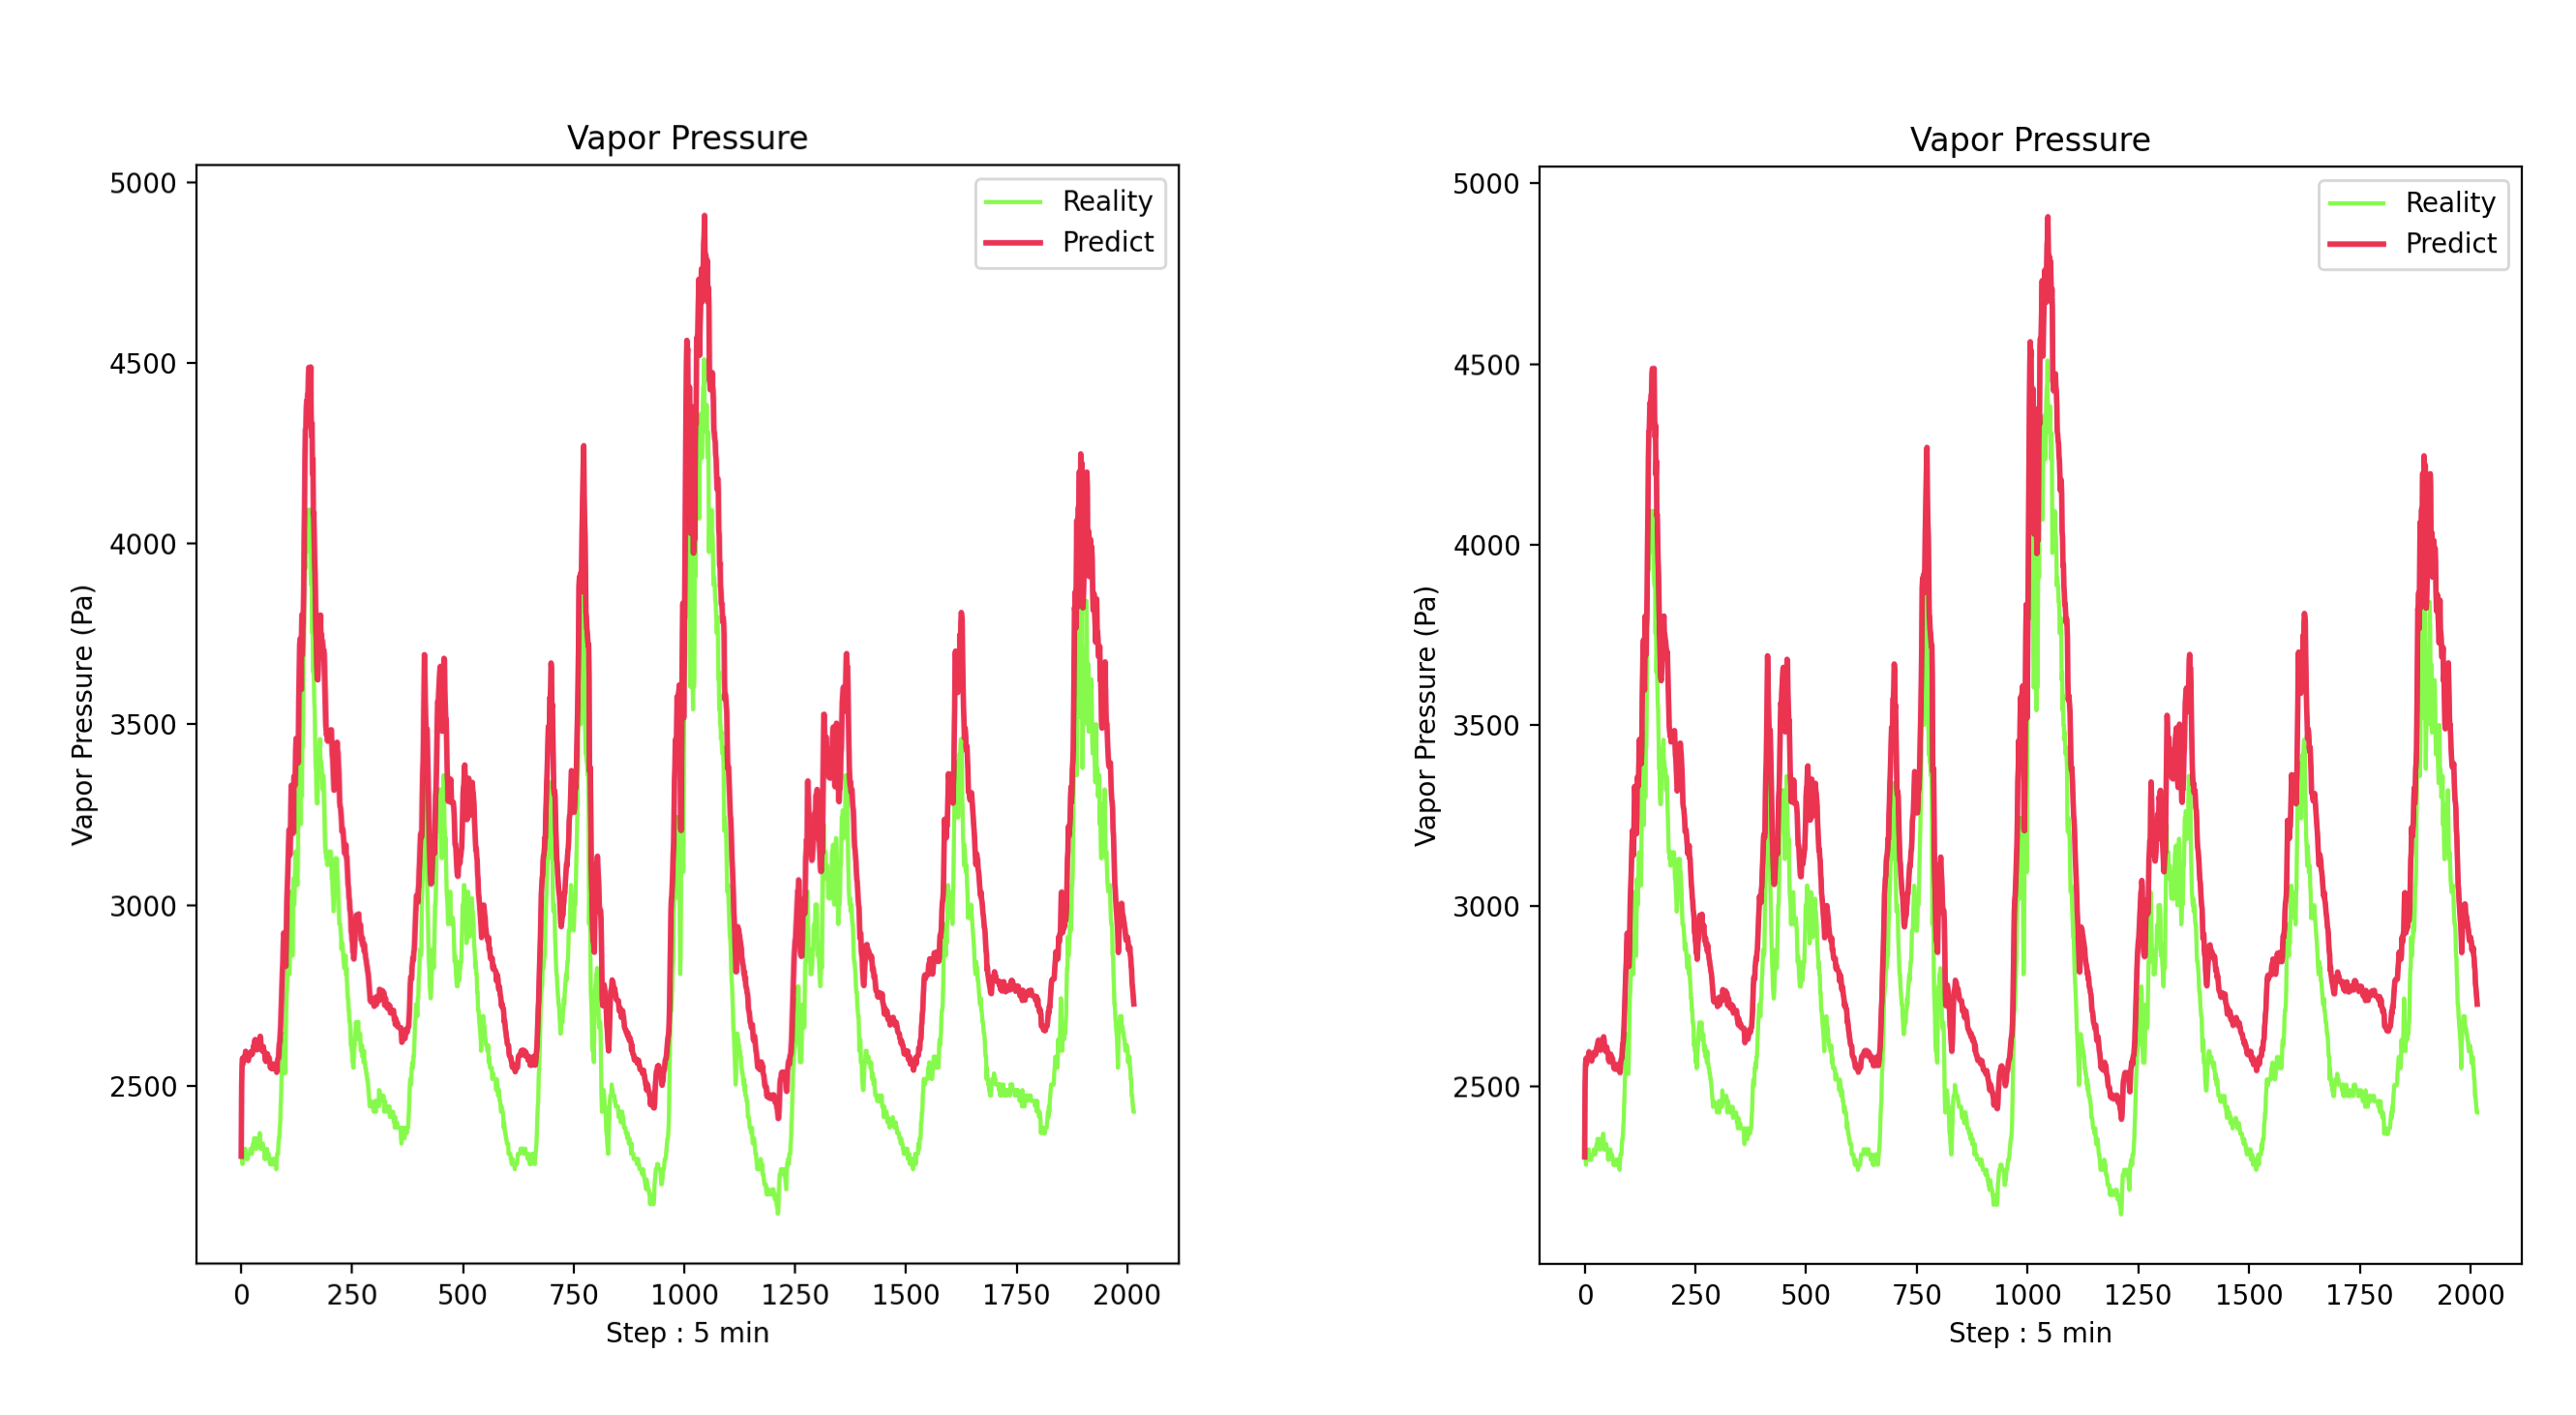
\includegraphics[width=\textwidth]{VP_compare.png}
  \caption{\( VP \) values approximation using Euler method (left) and fourth-order Runge-Kutta method (right)}
\end{figure}

The Euler's method and fourth-order Runge-Kutta method yield nearly identical sets of values. The \( RMSE \) of this calculation using Euler's method is \( 315.3542\ Pa \), and using Runge-Kutta's is \( 315.3341\ Pa \). The values are obtained with high accuracy compared to the actual data, so our model is capable of simulating the change in vapor pressure of water of the given greenhouse model.

\newpage
%%%%%%%%%%%%%%%%%%%%%%%%%%%%%%%%%
\section{(Bonus exercise) Applying deep learning models}
\subsection{An approach to solving a simple ODE model}
%Introduction
In the previous chapters, we have solved ordinary differential equations (ODE) using finite-difference methods, which are Euler and Runge-Kutta schemes. However, these methods have some limitations, such as accumulating the approximation errors, since it depends on the result of the previous step, and taking up a huge amount of space to store the result. Therefore, in this chapter, we will explore the techniques in Deep Learning to solve ODE in a closed continuous analytical form. More specifically, we will use an artificial neural network (ANN) to tackle the problem.

\begin{figure}[H]
  \centering
  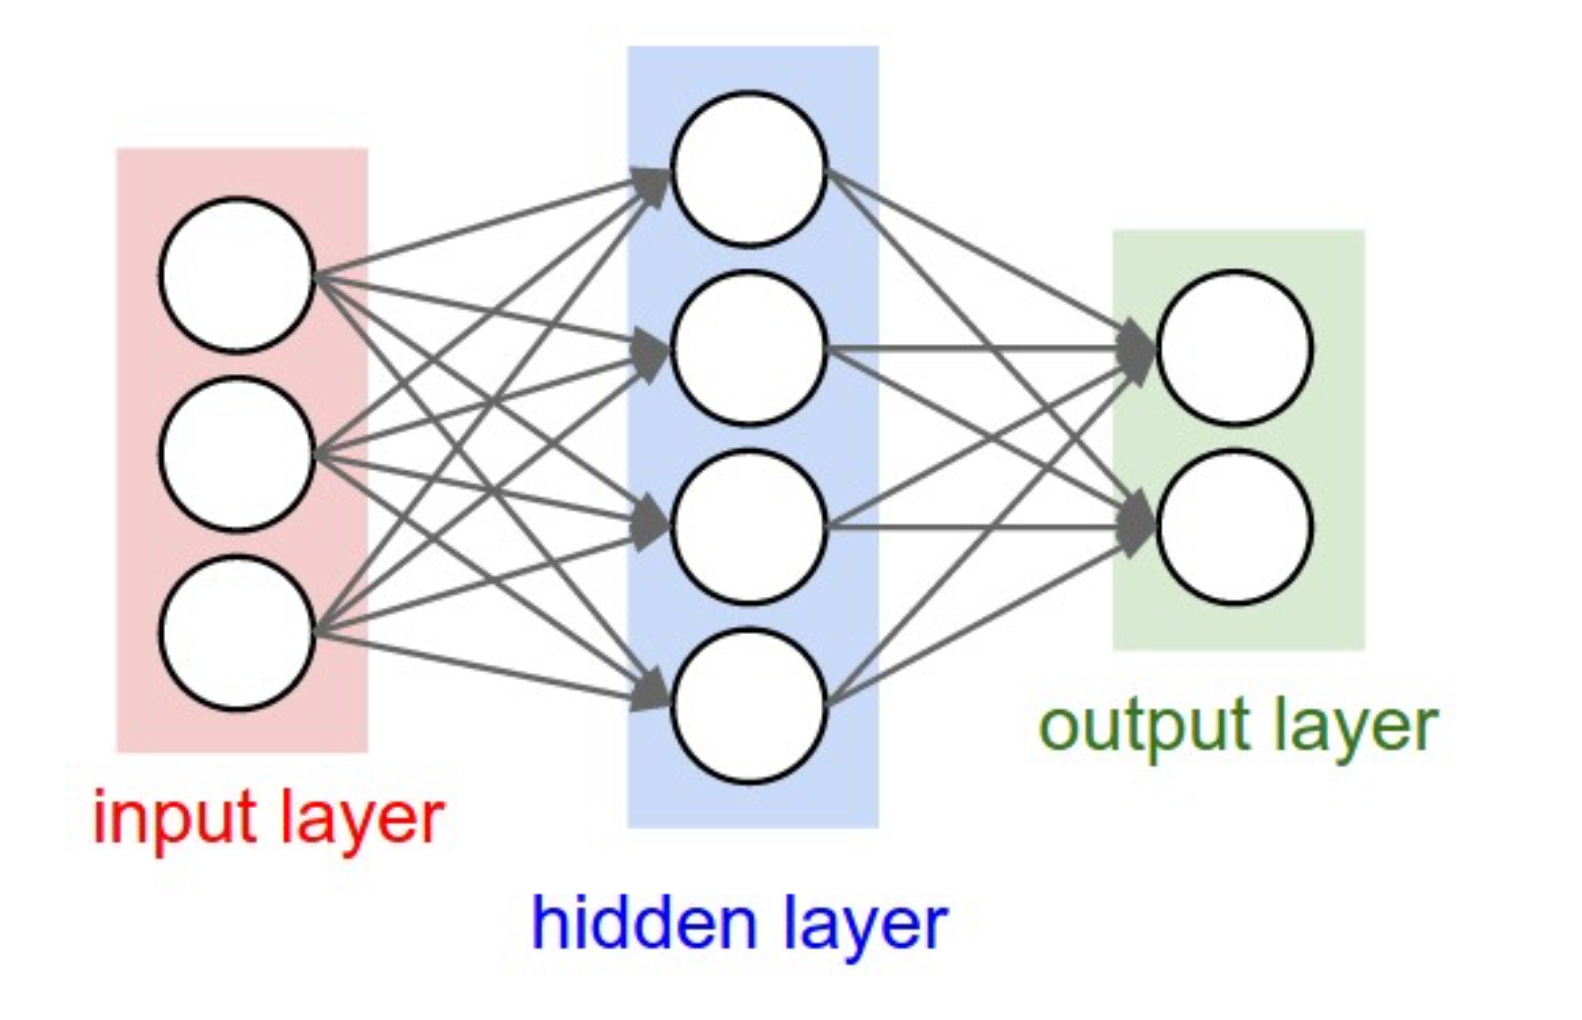
\includegraphics[width=\textwidth]{nn.png}
  \caption{Artificial neural network with 1 hidden layer}
\end{figure}

It was established that an ANN with only one hidden layer and a nonlinear activation function was capable of approximating any function. The solutions are stored as neural network parameters, which does not require as much memory as the previous methods. Our attempt is using feed-forward neural network to solve a simple ODE initial value problem. To evaluate the performance, we will then calculated the RMSE of the obtained values with the exact solutions that we have computed in Chapter 1.

% Intro to autograd
Deep Learning, the use of many-layered artificial neural networks very loosely based on ideas about computation in mammalian brains, is well known for its impacts on fields like computer vision and natural language processing.
Much of deep learning boils down to specifying a model by defining a scalar function of multiple parameters - a loss functions or a probability density - and optimizing or sampling from this model.
For such high-dimensional problems, gradients are indispensable.

Gradients, in principle, can always be computed automatically given the function itself.
Many different automatic differentiation packages for machine learning have been addressed.
However, the most commonly used packages, Theano\cite{bastien2012theano} and Torch\cite{collobert2002torch}, tend to have several drawbacks that make them difficult to use:
\begin{itemize}
  \item They require learning a new syntax in which to express basic operations, essentially acting as interpreters for a restricted mini-language.
  \item These mini-languages tend to have very limited control flow operations.
  \item These mini-languages tend to have limited support for array indexing and other helper functions.
\end{itemize}

\textbf{An algorithm to solve the general ODE model with the form:}
\begin{align*}
  \begin{cases}
    \dot{x}(t) = f(t, x), \\
    x(t_0) = x_0.
  \end{cases}
\end{align*}

\textbf{where \( f \) is a function depending on \( t \) and \( x(t) \) (\( x \) and \( f \) are vectors).}

The universal approximation theorem\cite{hornik89feedforward} states that any continuous function can be approximated by a feed-forward neural network with a single hidden layer. This ANN can be written in a matrix multiplication form:
\begin{align*}
  N(t; w) = W_2 \sigma (W_1 t + b_1) + b_2
\end{align*}

where \( W_1 \) and \( W_2 \) are weight matrices and \( b_1 \) and \( b_2 \) are bias terms. \( \sigma \) is a nonlinear activation function such as \( \tanh \). We use \( w \) to represent all parameters \( [W_1, W_2, b_1, b_2] \). To fit a scalar function \( x(t) \), the neural network takes a scalar input \( t \) and returns a scalar output \( N(t) \). In this case, \( W_1 \) and \( W_2 \) degrade to row and column vectors.

The optimal parameters \( w \) can be found by minimizing the loss function
\begin{align*}
  L(w) = \int_a^b {[x(t) - N(t; w)]}^2 dt
\end{align*}

In practice, the integral is approximated by a summation
\begin{align*}
  L(w) = \sum_i {[x(t_i) - N(t_i; w)]}^2
\end{align*}

where \( \{t_i\} \) is a set of training points covering the domain \( [a, b] \).

If the loss is small enough, then the ANN can be considered as a good approximation to the original function over the domain \( [a, b] \):
\begin{align*}
  N(t; w) \approx x(t)
\end{align*}

Now we consider constructing an ANN that can approximate the solution to the first-order ODE:
\begin{align*}
  \dot{x}(t) = f(t, x(t)),\ x(t_0) = x_0
\end{align*}

If we use a standard neural network
\begin{align*}
  N(t; w) = W_2\sigma(W_1t + b_1) + b_2
\end{align*}

It will not satisfy the initial condition, i.e. typically \( N(t_0; w) \neq x_0 \).  But we can force the initial condition by rewriting the ANN solution as
\begin{align*}
  \hat{x}(t; w) = x_0 + (t - t_0)N(t; w)
\end{align*}

For any parameters \( w \) , there will always be \( \hat{x}(t_0; w) = x_0 \). We further require this ANN solution \( \hat{x}(t; w) \) to satisfy the ODE:
\begin{align*}
  \dot{\hat{x}}(t; w) \approx f(t, \hat{x}(t; w))
\end{align*}

Note that the derivative \( \dot{\hat{x}}(t; w) \) can be derived analytically without any finite-difference approximation
\begin{align*}
  \dot{\hat{x}}(t; w) = \frac{\partial [x_0 + (t - t_0)N(t; w)]}{\partial t} = \frac{\partial (t - t_0)}{\partial t}N(t; w) + (t - t_0)\frac{\partial N(t; w)}{\partial t}
\end{align*}

The optimal parameters can be found by minimizing the cost function
\begin{align*}
  L(w) = \int_{t_0}^{t_1} [\dot{\hat{x}}(t; w) - f(t, \hat{x}(t; w)]^2 dt
\end{align*}

Or in practice,
\begin{align*}
  L(w) \approx \sum_i [\dot{\hat{x}}(t_i; w) - f(t_i, \hat{x}(t_i; w)]^2
\end{align*}

Where \( \{t_i\} \) is a set of training points covering the domain \( [t_0, t_1] \).

If the loss is small enough, then the ANN solution should be able to approximate the true ODE solution over the domain \( [t_0, t_1] \):
\begin{align*}
  \hat{x}(t; w) \approx x(t)
\end{align*}

Here the initial condition \( x_0 \) is fixed during the ANN training, which means we need to re-train the ANN for a new initial condition.

To build this ANN, \texttt{Autograd} is a project to bring automatic differentiation to Python, Numpy\cite{oliphant2007python} and Scipy\cite{jones2001scipy} code written using the facilities that this modern scientific computing framework offers.

\subsection{A simple deep learning model for a set of differential equations}
As described above, the ANN method to solve simple ODE, which is the primary goal, and then compare Neural Network results with traditional finite difference method which we treat as ground truth.

To test the stability of our ANN method, the ANN model is trained 2000 times (default Iteration times) and its histogram of performance is plotted over 2000 fittings. By observation, in most cases ANN method can approximate the ground truth well, whereas sometimes it requires increased amount of training the network to get ideal results.

The program used to implement this method is written in Python, which means in order to apply it to certain model users need to rewrite the method following the rules guarded by Python Programming Language.

\subsubsection{A simple ODE example}
To illustrate practical implementation of the deep learning model above, we consider this ODE with initial value as an example:
\begin{align*}
  \begin{cases}
    \frac{dy}{dt} & = \frac{-t}{y - 3} \\
    y(t_0)        & = 1
  \end{cases}
\end{align*}

Using Calculus, this ODE can be solved and yields a unique solution:
\begin{align}
  y = 3 - \sqrt{4-t^2}
\end{align}

Firstly, we must define an ODE function that is comprehensible for the program. Considering the example above, the function is constructed as:
\begin{mdframed}[leftline=false,rightline=false,backgroundcolor=magenta!10,nobreak=true]
  \begin{minted}[linenos,breaklines,breaksymbolleft=,obeytabs=true,tabsize=2]{Python}
def f(t, y):
    '''
        dy/dt = f(t, y)
        This is f() function on the right
    '''
    return [-t/(y[0] - 3)] # should be a list
  \end{minted}
\end{mdframed}

\subsubsection{Building the model}
To build a model, we can declare an object assigned to the class that is responsible for the deep learning model:
\begin{mdframed}[leftline=false,rightline=false,backgroundcolor=magenta!10,nobreak=true]
  \begin{minted}[linenos,breaklines,breaksymbolleft=,obeytabs=true,tabsize=2]{Python}
t = np.linspace(-2, 2, 100).reshape(-1,1)
y0_list = [1] # should be a list
nn = NNSolver(f, t, y0_list)
nn
  \end{minted}
\end{mdframed}

With \texttt{f} is the function we defined above, \texttt{t} is input of the function \( y(t) \), \texttt{y0\_list} is the value at initial state of the ODE. Using \texttt{nn} in the second line of the code will print the current state of the model we just declared:
\begin{mdframed}[leftline=false,rightline=false,backgroundcolor=Turquoise!10,nobreak=true]
  \begin{minted}[breaklines,breaksymbolleft=,obeytabs=true,tabsize=2]{Python}
Neural ODE Solver
Number of equations:       1
Initial condition y0:      [1]
Number of hidden units:    10
Number of training points: 100
    \end{minted}
\end{mdframed}

\subsubsection{Training the model}
To train the model, first we will need to reset all the weights inside. We can do that through an implemented method in the model called \texttt{reset\_weights()}. Then we can call \texttt{train()} which is used to train our model.
\begin{mdframed}[leftline=false,rightline=false,backgroundcolor=magenta!10,nobreak=true]
  \begin{minted}[linenos,breaklines,breaksymbolleft=,obeytabs=true,tabsize=2]{Python}
nn.reset_weights()
nn.train()
    \end{minted}
\end{mdframed}
Screen output:
\begin{mdframed}[leftline=false,rightline=false,backgroundcolor=Turquoise!10,nobreak=true]
  \begin{minted}[breaklines,breaksymbolleft=,obeytabs=true,tabsize=2]{Python}
iteration: 0 loss:  4.386270987155103
iteration: 200 loss:  0.008455467990056757
iteration: 400 loss:  0.005912794671912592
iteration: 600 loss:  0.005269032339101694
iteration: 800 loss:  0.004350997334545889
iteration: 1000 loss:  0.003384068549831591
iteration: 1200 loss:  0.0029158045232204255
iteration: 1400 loss:  0.0023676879422605953
iteration: 1600 loss:  0.001876234320686411
iteration: 1800 loss:  0.0016967184483936597
Warning: Maximum number of iterations has been exceeded.
         Current function value: 0.001653
         Iterations: 2000
         Function evaluations: 2264
         Gradient evaluations: 2264
    \end{minted}
\end{mdframed}
With the default limit of iterations is 2000, we can observe the result at the screen. We can extract the value of the method as shown below to visualize the exact value of loss function:
\begin{mdframed}[leftline=false,rightline=false,backgroundcolor=magenta!10,nobreak=true]
  \begin{minted}[linenos,breaklines,breaksymbolleft=,obeytabs=true,tabsize=2]{Python}
nn.loss_func(nn.params_list)
    \end{minted}
\end{mdframed}
Value output: 0.001652800015919836

\subsubsection{Comparing the ANN method to the actual function}
The code below is used to plot two functions at the same time:
\begin{mdframed}[leftline=false,rightline=false,backgroundcolor=magenta!10,nobreak=true]
  \begin{minted}[linenos,breaklines,breaksymbolleft=,obeytabs=true,tabsize=2]{Python}
y_pred_list, _ = nn.predict()
plt.plot(t, 3 - (4 - t**2)**0.5, label='true') # Real data
plt.plot(t, y_pred_list[0], 'o', label='y1 predict') # Predict data
plt.legend()
    \end{minted}
\end{mdframed}
Screen output:
\begin{figure}[H]
  \centering
  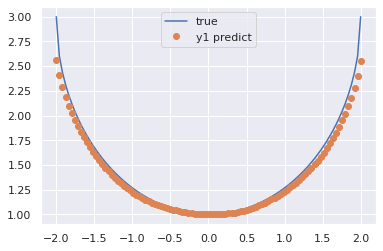
\includegraphics[width=0.7\textwidth]{ODEplot.png}
  \caption{Figure of actual functions and ANN method}
\end{figure}

To measure the accuracy of the model, we can use root mean square to calculate the total difference of two functions. The code below is used for calculating root mean square:
\begin{mdframed}[leftline=false,rightline=false,backgroundcolor=magenta!10,nobreak=true]
  \begin{minted}[linenos,breaklines,breaksymbolleft=,obeytabs=true,tabsize=2]{Python}
N = len(t)
RMSE = 0
for real, predict in zip(3 - (4 - t**2)**0.5, y_pred_list[0]):
  RMSE += (real - predict) ** 2
RMSE = (RMSE/N) ** (1 / 2)
print("Root Mean Squared Error: ", RMSE)
    \end{minted}
\end{mdframed}
Screen output:
\begin{mdframed}[leftline=false,rightline=false,backgroundcolor=Turquoise!10,nobreak=true]
  \begin{minted}[breaklines,breaksymbolleft=,obeytabs=true,tabsize=2]{Python}
Root Mean Squared Error:  [0.08718057]
    \end{minted}
\end{mdframed}

\subsubsection{Conclusion}
Through observation, we see that the root mean square error is not too large. This means that this model predicts with decent accuracy and can be practically used.


\newpage

\printbibliography[heading=bibintoc]

\end{document}
